\documentclass{article}
\usepackage[utf8]{inputenc}
\usepackage{graphicx}
\usepackage[version=4]{mhchem}

% additional packages
\usepackage{color}
\usepackage{siunitx}
\usepackage{amssymb}
\usepackage{booktabs}
\usepackage{threeparttable}

% Units

\DeclareSIUnit{\angstrom}{\text{\AA}}

% References and abbreviations
\newcommand*{\eg}{\emph{e.g. }}
\newcommand*{\etal}{\emph{et al.}}
\newcommand*{\ie}{\emph{i.e. }}
\newcommand*{\reffig}[1]{Fig.~\ref{#1}}
\newcommand*{\refsec}[1]{Section~\ref{#1}}
\newcommand*{\refeq}[1]{Eq.~\ref{#1}}
\newcommand*{\reftab}[1]{Table.~\ref{#1}}

% Symbols for physics
\newcommand*{\dcp}{d_{\mathrm{cp}}}
\newcommand*{\phieff}{\phi_{\mathrm{eff}}}
\newcommand*{\dsg}{d_{\mathrm{sg}}}
\newcommand*{\dion}{d_{\mathrm{ion}}}
\newcommand*{\deff}{d_{\mathrm{eff}}}
\newcommand*{\nsg}{N_{\mathrm{sg}}}
\newcommand*{\npp}{N_{\mathrm{PP}}}
\newcommand*{\nnp}{N_{\mathrm{NP}}}
\newcommand*{\qpp}{q_{\mathrm{PP}}}
\newcommand*{\qnp}{q_{\mathrm{NP}}}
\newcommand*{\nup}{N_{\mathrm{UP}}}
\newcommand*{\qup}{q_{\mathrm{UP}}}
\newcommand*{\qp}{q_{\mathrm{p}}}
\newcommand*{\np}{N^{\mathrm{p}}}
\newcommand*{\npsg}{N^{\mathrm{p}}_{\mathrm{sg}}}
\newcommand*{\pnpsg}{P^{\np}_{\npsg}}
\newcommand*{\pzz}{P^{0}_{0}}
\newcommand*{\poe}{P^{1}_{8}}
\newcommand*{\pte}{P^{2}_{8}}
\newcommand*{\pn}{P^\mathrm{n}}
\newcommand*{\lbox}{L_\mathrm{box}}
\newcommand*{\vp}{\phi_\mathrm{p}}
\newcommand*{\nmi}{N_{\mathrm{mi}}}
\newcommand*{\ncl}{N_{\ce{Cl-}}}
\newcommand*{\nna}{N_{\ce{Na+}}}
\newcommand*{\acl}{a_{\ce{Cl-}}}
\newcommand*{\ana}{a_{\ce{Na+}}}
\newcommand*{\anacl}{a_{\ce{NaCl}}}
\newcommand*{\ccl}{c_{\ce{Cl-}}}
\newcommand*{\cna}{c_{\ce{Na+}}}
\newcommand*{\gpm}{\gamma_{\pm}}
\newcommand*{\dpex}{\Delta p_\mathrm{excess}}
\newcommand*{\dptot}{\Delta p^\mathrm{osm}_\mathrm{total}}
\newcommand*{\dpid}{\Delta p_\mathrm{ideal}}
\newcommand*{\pex}{p_\mathrm{excess}}
\newcommand*{\ptot}{p^\mathrm{osm}_\mathrm{total}}
\newcommand*{\pid}{p_\mathrm{ideal}}
\newcommand*{\dl}{\kappa^{-1}}
\newcommand*{\bulk}{\mathrm{bulk}}
\newcommand*{\neutral}{\mathrm{neutral}}
\newcommand*{\cppm}{\mathrm{CPPM}}
\newcommand*{\csalt}{c_\mathrm{salt}}

% ── Cross-reference to main document ──────────────────────────────────────────
% Requires main.aux to exist (compile main.tex before esi.tex).
% All labels from main.tex are accessible without prefix.
\usepackage{xr}
\externaldocument{main}

% ── ESI-style numbering ───────────────────────────────────────────────────────
\renewcommand{\thefigure}{S\arabic{figure}}
\renewcommand{\thetable}{S\arabic{table}}
\renewcommand{\thesection}{S\arabic{section}}
\renewcommand{\thesubsection}{S\arabic{section}.\arabic{subsection}}
\setcounter{figure}{0}
\setcounter{table}{0}
\setcounter{section}{0}

\title{Supporting Information\\[0.5ex]
\large Ion Asymmetry and Electrostatic Screening in Dense Solutions of Patchy Macroions}

\author{Sebastian Pineda, Mikael Lund}
\date{}

\begin{document}

\maketitle

\tableofcontents

\bigskip\noindent
This document contains six sections of supporting information for the main article.
Figures and tables are numbered S1, S2, \ldots and sections S1, S2, \ldots\
Cross-references to the main article are typeset as, e.g., ``main Fig.~\ref{fig:gofr_exp}''
or ``main Sec.~\ref{sec:struc_ana}''.

% ─────────────────────────────────────────────────────────────────────────────
\section{Simulation details\label{esi:sec:simdetails}}
% ─────────────────────────────────────────────────────────────────────────────

\begin{figure}[htbp]
    \centering
    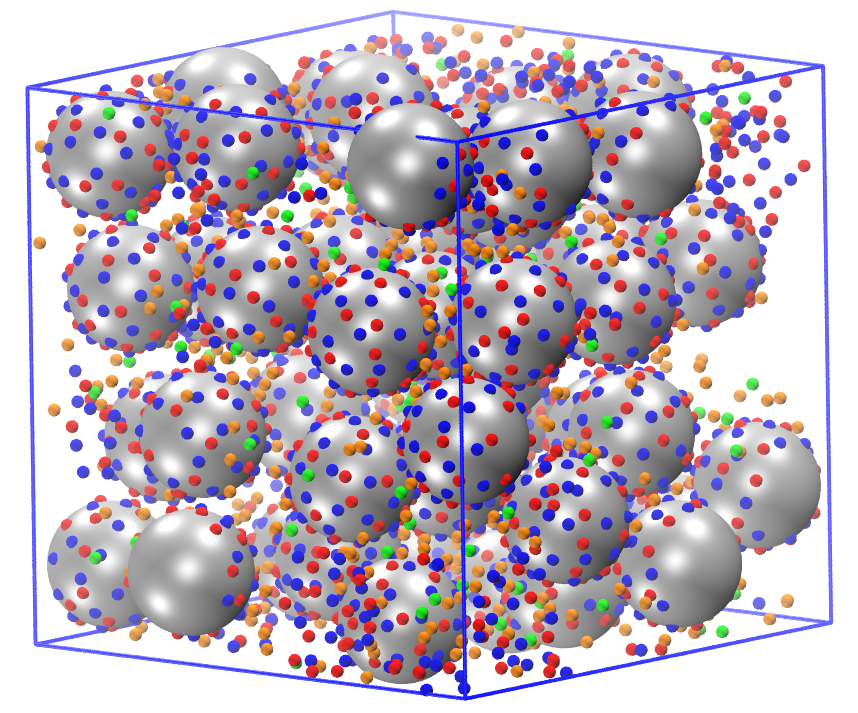
\includegraphics[height=0.5\textwidth]{figs/sim_box_2.png}
    \caption{Simulation snapshot of the isotropic CPPM variant ($\pzz$) in a periodic cubic box at volume fraction $\vp = 0.30$ with \ce{NaCl} ions at constant activity $\anacl = \qty{100}{mM}$.
    Color coding: gray = center particle, red = positive surface groups, blue = negative surface groups, orange = sodium ions, green = chloride ions.}
    \label{fig:snapshot}
\end{figure}

\subsection{Simulation system}

All systems consisted of $\nmi = 30$ rigid macro-ions in a cubic simulation box of side length $\lbox = \qty{149.64}{\angstrom}$, corresponding to a macro-ion volume fraction of $\vp = 0.30$.
The solvent was modeled as a dielectric continuum with the permittivity of water at $T = \qty{298.15}{\kelvin}$, $\varepsilon_r = 78.36$.

\paragraph{Explicit-ion simulations.}

Monovalent sodium and chloride ions were included explicitly alongside the macro-ions.
They were modeled as charged spherical beads of diameter $\dion = \qty{4}{\angstrom}$ and elementary charge $\pm e$.
Their chemical potential was controlled by grand-canonical Monte Carlo (GCMC) insertion/deletion of \ce{Na+} and \ce{Cl-} pairs targeting a reference salt activity of $\ana = \acl = \qty{0.1}{M}$, with zero free-energy bias.
For the three charged macro-ion variants the boxes initially accommodated $\nna = 300$ sodium and $\ncl = 60$ chloride ions on average.
For the neutral variant, $\nna = \ncl = 123$ ions of each species were used to maintain electroneutrality.
Those specific numbers were chosen based on preliminary simulations.
A reference electrolyte simulation (bulk) was carried out in the same box without macro-ions.

\paragraph{Implicit-ion simulations.}

Implicit-ion simulations replaced the explicit ions with a Debye--Hückel screening term, parameterized by the Debye screening length $\dl$ (main \refeq{eq:yukawa}).
Simulations were performed over the $\dl$ ranges listed in main \reftab{tab:kappa}.
For each charged variant, an additional simulation was run at $\dl_\mathrm{th} = \qty{9.61}{\angstrom}$ corresponding to an ionic strength of $I = \qty{0.1}{M}$~\cite{israelachvili2011}.

\paragraph{Interaction potentials.}

Electrostatic interactions were evaluated with the Fanourgakis real-space, charge-neutral method~\cite{fanourgakis2009} with a spherical cutoff $r_c = \lbox/2 = \qty{74.82}{\angstrom}$.
In the explicit-ion simulations the full Coulomb potential was used; in the implicit-ion simulations it was multiplied by the Debye--Hückel factor to give the Yukawa potential (main \refeq{eq:yukawa}).
Short-range repulsions between all bead pairs were modeled with the Weeks--Chandler--Andersen (WCA) potential using Lorentz--Berthelot combining rules and well depth $\varepsilon = \qty{2.479}{\kilo\joule\per\mol}$ ($= k_{\rm B}T$ at \qty{298.15}{\kelvin}).

\subsection{Simulation protocol}

Configurations were sampled with the Metropolis criterion over $4\times10^4$ macro-steps.
Each macro-step combined:
(i) rigid-body translation ($\Delta r_{\max} = \qty{4.0}{\angstrom}$) and rotation ($\Delta\theta_{\max} = \qty{0.4}{\radian}$) trials for each macro-ion;
(ii) preferential-sampling translations of the explicit ions biased towards macro-ion surfaces with weight $W(r) \propto (r + \qty{5}{\angstrom})^{-2}$ and maximum displacement $\qty{14}{\angstrom}$; and
(iii) GCMC insertion/deletion attempts for neutral \ce{Na+}--\ce{Cl-} pairs.
In the implicit-ion runs only moves of type~(i) were applied.
Three independent replicas were run for each variant and $\dl$ value; all reported quantities are mean $\pm$ standard error across replicas.

\subsection{Analysis}

\paragraph{Radial distribution function.}

CPPM--CPPM radial distribution functions $g(r)$ were computed from centers of mass every 10 MC steps (resolution \qty{0.25}{\angstrom}).
The analytical Percus--Yevick (PY) hard-sphere $g(r)$ was computed as a theoretical reference.
The PY structure factor $S(q)$ was evaluated on 50,000 uniformly spaced $q$-points up to $q_\mathrm{max} = \qty{5.0}{\angstrom}$ using the exact Wertheim--Thiele solution \cite{Wertheim1963,Thiele1963}.
The pair distribution function was obtained via the sine transform
\begin{equation}
      g(r) - 1 = \frac{1}{2\pi^2\rho} \int_0^{q_\mathrm{max}} q^2\bigl[S(q)-1\bigr]\frac{\sin(qr)}{qr} \mathrm{d}q,
\end{equation}
with a Lorch window $W(q) = \sin(\pi q/q_\mathrm{max})/(\pi q/q_\mathrm{max})$ applied to suppress Gibbs truncation artifacts.
The effective hard-sphere diameter $\deff$ was fitted to the neutral CPPM $g(r)$ by minimizing the root-mean-square deviation of $f(r) = g(r)\cdot r^2$; the effective volume fraction follows as $\phieff = \vp(\deff/\dcp)^3$.

In addition to CPPM--CPPM distribution functions, ion--CPPM pair distributions (\ce{Na+}--NP, \ce{Cl-}--PP, \ce{Na+}--MP, \ce{Cl-}--MP) were computed in the explicit-ion runs.
A correction for the partial occlusion of each spherical shell by the macro-ion was applied for $r < \deff = \dcp + \dsg = \qty{44}{\angstrom}$ by dividing by the accessible shell fraction $f_\text{acc}(r) = (\deff + r)/(2\,\deff)$.
The \ce{Na+}--\ce{Cl-} pair distribution was also computed, including the bulk \ce{NaCl} reference.

\paragraph{Optimal screening-length selection.}

For each charged variant, the quality of each implicit-ion $g(r)$ was assessed by the peak absolute deviation $|\Delta g|_\text{max}$ against the explicit-ion reference, restricted to $r \geq \qty{40.0}{\angstrom}$ to focus on medium- to long-range structure.
The $\dl$ value minimizing $|\Delta g|_\text{max}$ was identified as $\dl_*$; to improve precision beyond the discrete grid the $|\Delta g|_\text{max}(\dl)$ curve was interpolated with a cubic spline and minimized on 10,000 points spanning the simulated range.

\paragraph{Multipole energy decomposition.}

Pairwise CPPM--CPPM interaction energies were decomposed as a function of center-of-mass separation $r$ using the Multipole Distribution analysis implemented in Faunus (resolution \qty{0.25}{\angstrom}, sampled every 10~steps).
For each configuration, the exact energy $u_\text{exact}$ (full bead--bead Coulomb sum) and the truncated multipole-expanded total $u_\text{tot} = u_{ii} + u_{id} + u_{dd} + u_{iq}$ (main Eqs.~\ref{eq:u_ii}--\ref{eq:u_iq}) were recorded.
The same analysis yielded orientational correlation functions as a function of $r$:
(a)~dipole--dipole correlation $\langle\hat{\mu}_i\cdot\hat{\mu}_j\rangle$;
(b)~longitudinal dipole projection $\langle(\hat{\mu}_i\cdot\hat{r}_{ij})(\hat{\mu}_j\cdot\hat{r}_{ij})\rangle$;
(c)~quadrupole--quadrupole correlation $\langle\hat{\mathbf{Q}}_i{:}\hat{\mathbf{Q}}_j\rangle$; and
(d)~nematic order parameter $\langle P_2(\cos\theta_{ij})\rangle = \langle(3\cos^2\theta_{ij}-1)/2\rangle$.

\paragraph{Spatial distribution functions.}

Three-dimensional density maps of surface beads (NP, PP) and explicit ions (\ce{Na+}, \ce{Cl-}) around the macro-ion reference frame were accumulated every 10 steps at \qty{1.5}{\angstrom} resolution with \qty{8}{\angstrom} padding and projected onto the unit sphere as Mollweide equal-area maps.

\paragraph{Osmotic pressure and activity coefficient.}

The total osmotic pressure $\ptot = \pid + \pex$ comprises ideal and excess contributions.
In the explicit-ion simulations the ideal part follows from the mean number densities of macro-ions, \ce{Na+}, and \ce{Cl-}.
In the implicit-ion runs, the ideal contribution reduces to the macro-ion number density alone.
The mean activity coefficient is estimated as $\gpm = \sqrt{\gamma_+\gamma_-} = \sqrt{a_+/c_+\cdot a_-/c_-}$.
The excess contribution was sampled by virtual isotropic volume perturbations ($\delta V = \qty{0.1}{\cubic\angstrom}$, block size 1000 steps).
The total osmotic pressure increment is computed as $\dptot = \ptot - p^{\mathrm{osm},\text{bulk}}_\mathrm{total}$.

% ─────────────────────────────────────────────────────────────────────────────
\section{Orientational correlation analysis\label{esi:sec:orient_ana}}
% ─────────────────────────────────────────────────────────────────────────────

\begin{figure}[htbp]
    \centering
    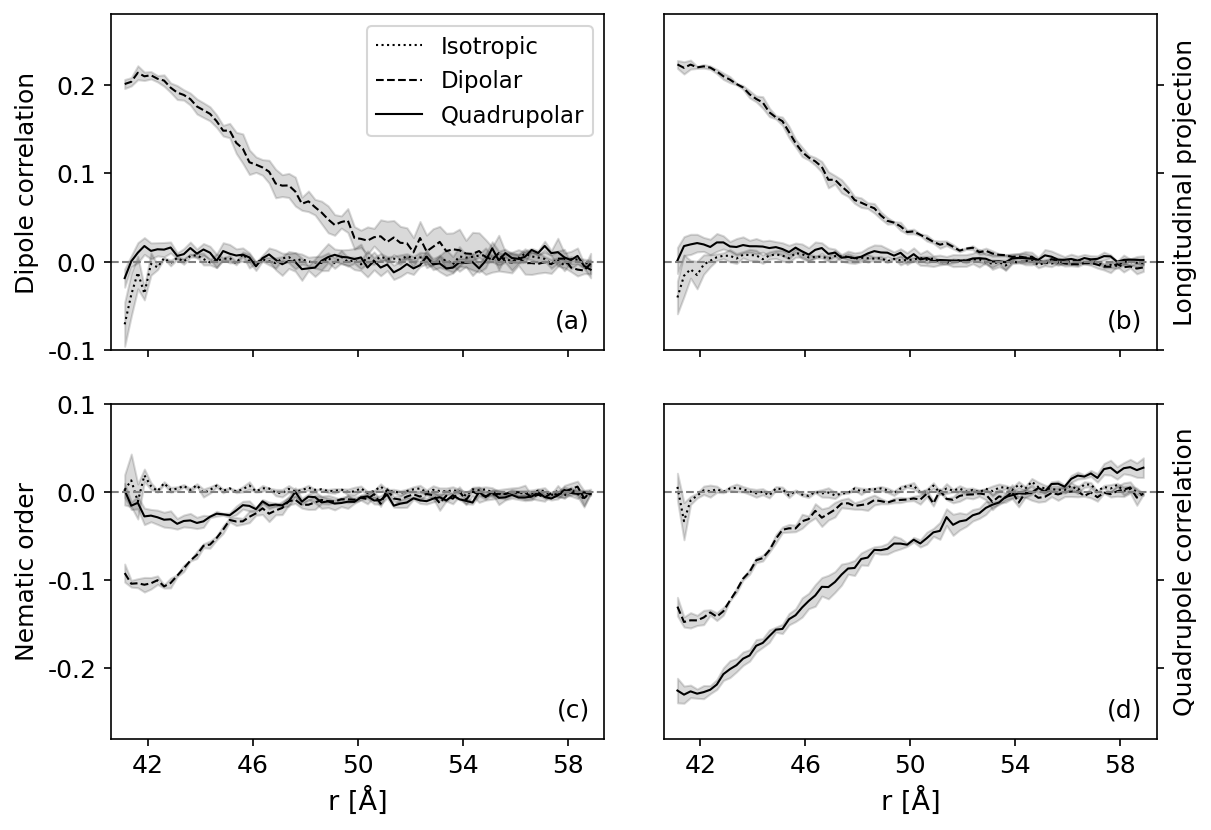
\includegraphics[width=\textwidth]{figs/multipole_corr_explicit_black.png}
    \caption{Distance-dependent orientational pair correlations between macro-ions for
    the three charged variants $\pzz$ (dotted), $\poe$ (dashed), and $\pte$ (solid)
    as a function of center-of-mass separation $r$.
    (a)~Dipole--dipole correlation $\langle\hat{\mu}_i\cdot\hat{\mu}_j\rangle$;
    (b)~longitudinal dipole projection
        $\langle(\hat{\mu}_i\cdot\hat{r}_{ij})(\hat{\mu}_j\cdot\hat{r}_{ij})\rangle$;
    (c)~nematic order parameter
        $\langle P_2(\cos\theta_{ij})\rangle=(3\cos^2\theta_{ij}-1)/2$;
    (d)~quadrupole--quadrupole correlation $\langle\hat{\mathbf{Q}}_i{:}\hat{\mathbf{Q}}_j\rangle$.
    Shaded bands: mean $\pm$ SEM across replicas.
    Horizontal gray line: uncorrelated reference ($= 0$).}
    \label{fig:multi_corr_exp}
\end{figure}

The isotropic variant $\pzz$ shows no significant orientational order at any separation
($|\text{correlation}| < 0.02$ for all four metrics), confirming that packing effects —
not electrostatic anisotropy — control the structure of this system, consistent with the
hard-sphere-like $g(r)$ discussed in main Sec.~\ref{sec:struc_ana}.

The dipolar $\poe$ exhibits a clear positive dipole--dipole correlation
($\langle\hat{\mu}_i\cdot\hat{\mu}_j\rangle \approx 0.17$ at $r \approx \qty{44}{\angstrom}$)
and an equally significant positive longitudinal projection ($\approx 0.19$), indicating that
neighboring dipolar macro-ions tend to adopt a head-to-tail configuration — the energetically
preferred arrangement for two interacting dipoles at close range.
The negative nematic order parameter ($\langle P_2 \rangle \approx -0.06$) is consistent with
a broad angular distribution where the head-to-tail motif dominates but perpendicular
configurations also occur.
The quadrupole--quadrupole correlation of $\poe$ is small and negative ($\approx -0.085$);
the primary orientational signature is dipolar.
All correlations in $\poe$ decay to noise by $r \approx \qty{52}{\angstrom}$, indicating that
orientational memory is confined to the contact shell.

The quadrupolar $\pte$ shows negligible dipole--dipole correlation ($< 0.01$) but a large
negative quadrupole--quadrupole correlation
($\langle\hat{\mathbf{Q}}_i{:}\hat{\mathbf{Q}}_j\rangle \approx -0.19$ at
$r \approx \qty{44}{\angstrom}$), indicating dominant anti-aligned quadrupolar ordering at
contact: the two positive patches of one macro-ion face the regions of highest negative charge
density on its neighbor.
The quadrupole correlation decays more slowly than the dipole correlations in $\poe$,
persisting to $r \approx \qty{55}{\angstrom}$, consistent with the slightly broader first-shell
peak in main Fig.~\ref{fig:gofr_exp}.

% ─────────────────────────────────────────────────────────────────────────────
\section{Multipole energy decomposition from explicit-ion simulations%
         \label{esi:sec:mpe}}
% ─────────────────────────────────────────────────────────────────────────────

\begin{figure}[htbp]
    \centering
    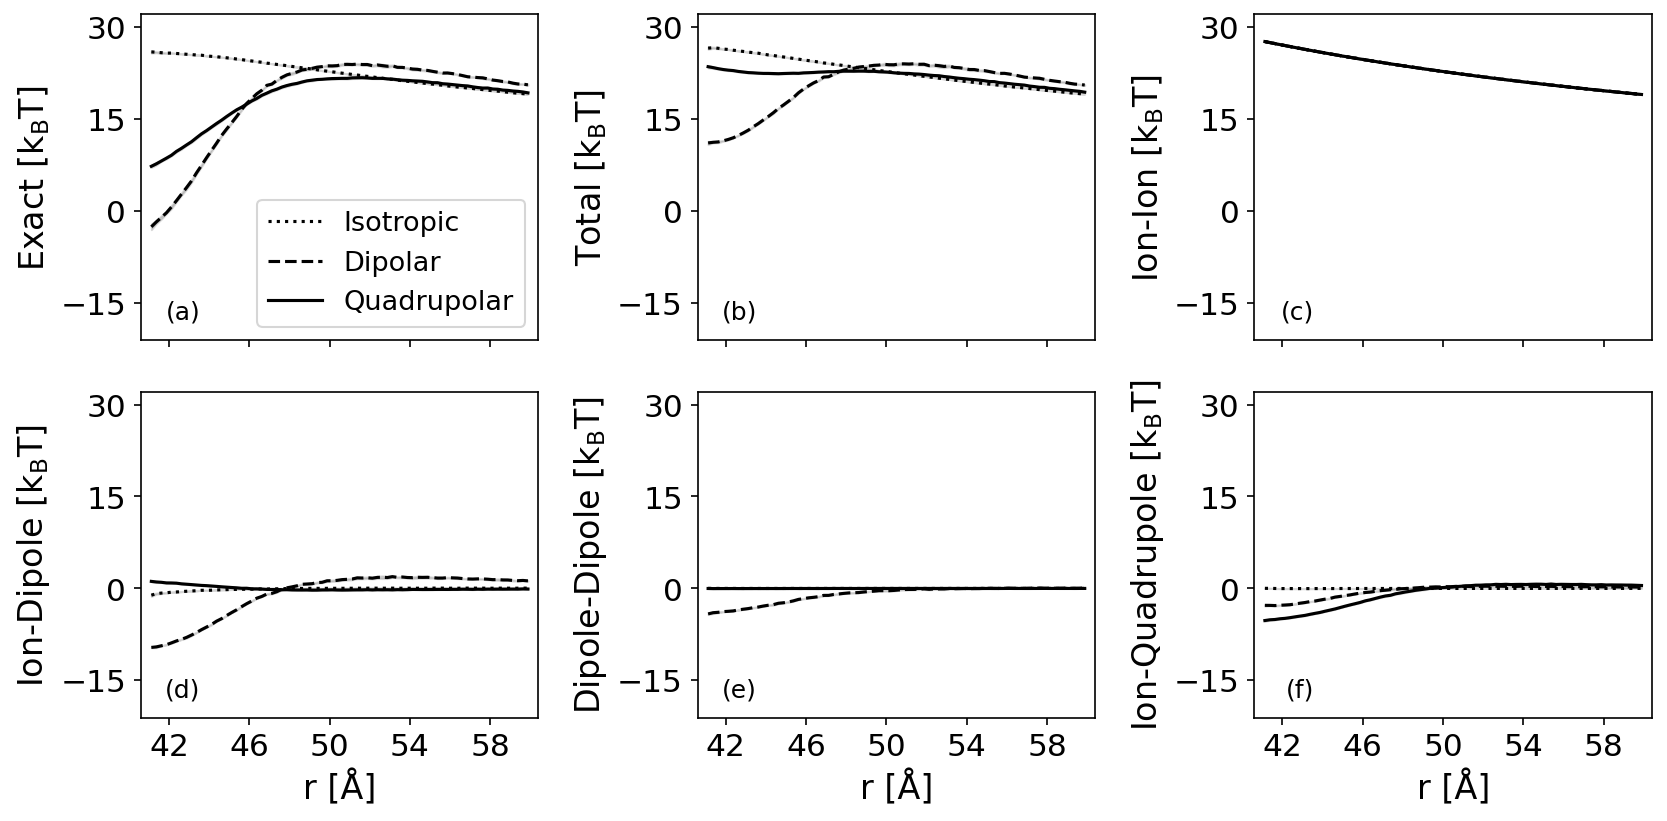
\includegraphics[width=\textwidth]{figs/multipole_energy_explicit_black.png}
    \caption{Distance-dependent pairwise energy contributions between macro-ions from
    explicit-ion simulations, for the three charged variants $\pzz$ (dotted),
    $\poe$ (dashed), and $\pte$ (solid) as a function of center-of-mass separation $r$.
    (a)~Exact total energy $u_\text{exact}$; (b)~multipole-expanded total $u_\text{tot}$;
    (c)~ion--ion $u_{ii}$; (d)~ion--dipole $u_{id}$;
    (e)~dipole--dipole $u_{dd}$; (f)~ion--quadrupole $u_{iq}$.
    Shaded bands: mean $\pm$ SEM across replicas.}
    \label{fig:multi_ene_exp}
\end{figure}

\reffig{fig:multi_ene_exp} compares the exact total pairwise energy $u_\text{exact}$
(full bead--bead Coulomb sum) against the truncated multipole-expanded total
$u_\text{tot} = u_{ii} + u_{id} + u_{dd} + u_{iq}$ (defined in main
Eqs.~\ref{eq:u_ii}--\ref{eq:u_iq}) as a function of pair separation.

For the isotropic $\pzz$ variant the two quantities agree to within $1.8\%$ at contact
($r \approx \qty{43}{\angstrom}$), and the fractional deviation falls below $0.1\%$ by
$r \approx \qty{48}{\angstrom}$.
This rapid convergence is expected: a nearly uniform charge distribution keeps the
higher-order multipole moments small, so the ion--ion term $u_{ii}$ dominates at all
relevant separations.

For the patchy variants the behavior is qualitatively different.
The dipolar $\poe$ shows a $275\%$ overestimate at contact ($u_\text{tot} \approx 12.6\,k_\mathrm{B}T$
vs.\ $u_\text{exact} \approx 3.3\,k_\mathrm{B}T$): in favorable head-to-tail configurations
the positive patch of one macro-ion faces the negative patch of its neighbor, producing a large
attractive higher-order contribution (dipole--quadrupole, quadrupole--quadrupole) that the
truncated expansion completely misses.
The error drops to $3.7\%$ at $r \approx \qty{48}{\angstrom}$ and below $0.2\%$ at
$r \approx \qty{52}{\angstrom}$.
The quadrupolar $\pte$ shows a $110\%$ overestimate at contact
($u_\text{tot} \approx 22.6\,k_\mathrm{B}T$ vs.\ $u_\text{exact} \approx 10.8\,k_\mathrm{B}T$)
and converges more slowly: a $10.6\%$ error persists at $r = \qty{48}{\angstrom}$ and
$< 1\%$ is not achieved until $r \approx \qty{60}{\angstrom}$.
The slower convergence for $\pte$ reflects the more spatially extended patch arrangement —
two patches separated by the particle diameter create a richer higher-order multipole
landscape that requires larger separations to enter the asymptotic regime.

These results demonstrate that the truncated multipole expansion is reliable only beyond
$r \approx 52$--$\qty{60}{\angstrom}$ (depending on anisotropy), well outside the
$\qty{44}{\angstrom}$ contact distance.
Within the first coordination shell — where structural and thermodynamic properties are
primarily determined — higher-order multipole terms make quantitatively significant
contributions for the patchy variants, underscoring the importance of the full bead--bead
Coulomb treatment in explicit-ion simulations.

% ─────────────────────────────────────────────────────────────────────────────
\section{Mollweide projections of the ion distribution on the CPPM surface%
         \label{esi:sec:mollweide}}
% ─────────────────────────────────────────────────────────────────────────────

\begin{figure}[htbp]
    \centering
    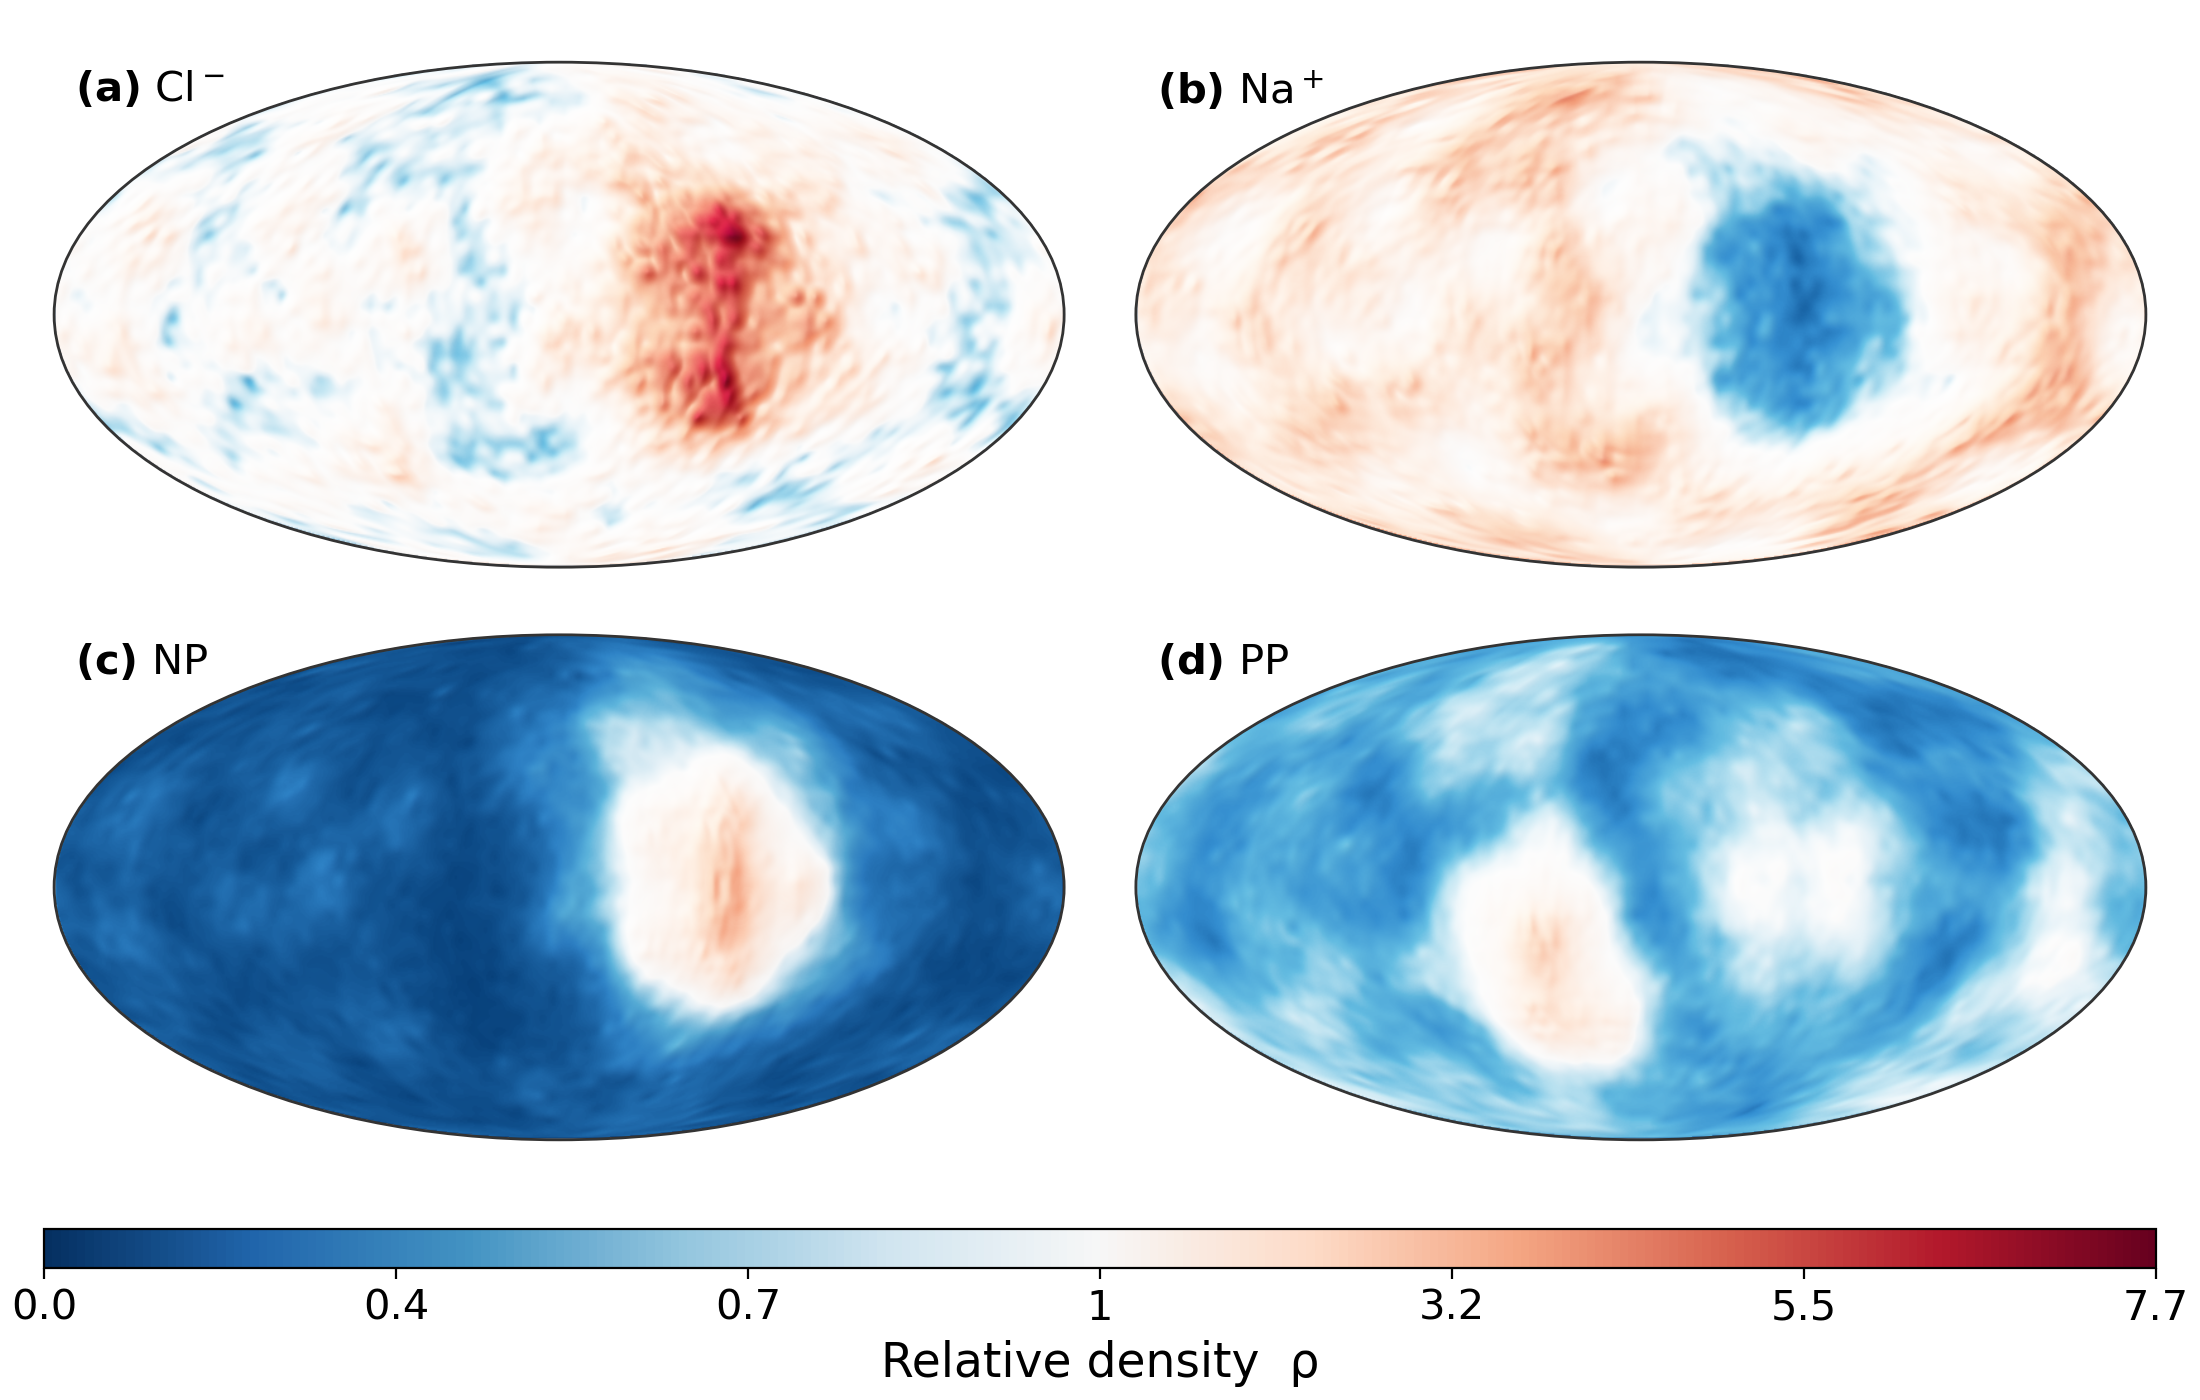
\includegraphics[width=\textwidth]{figs/dipolar-exp.png}\\[1em]
    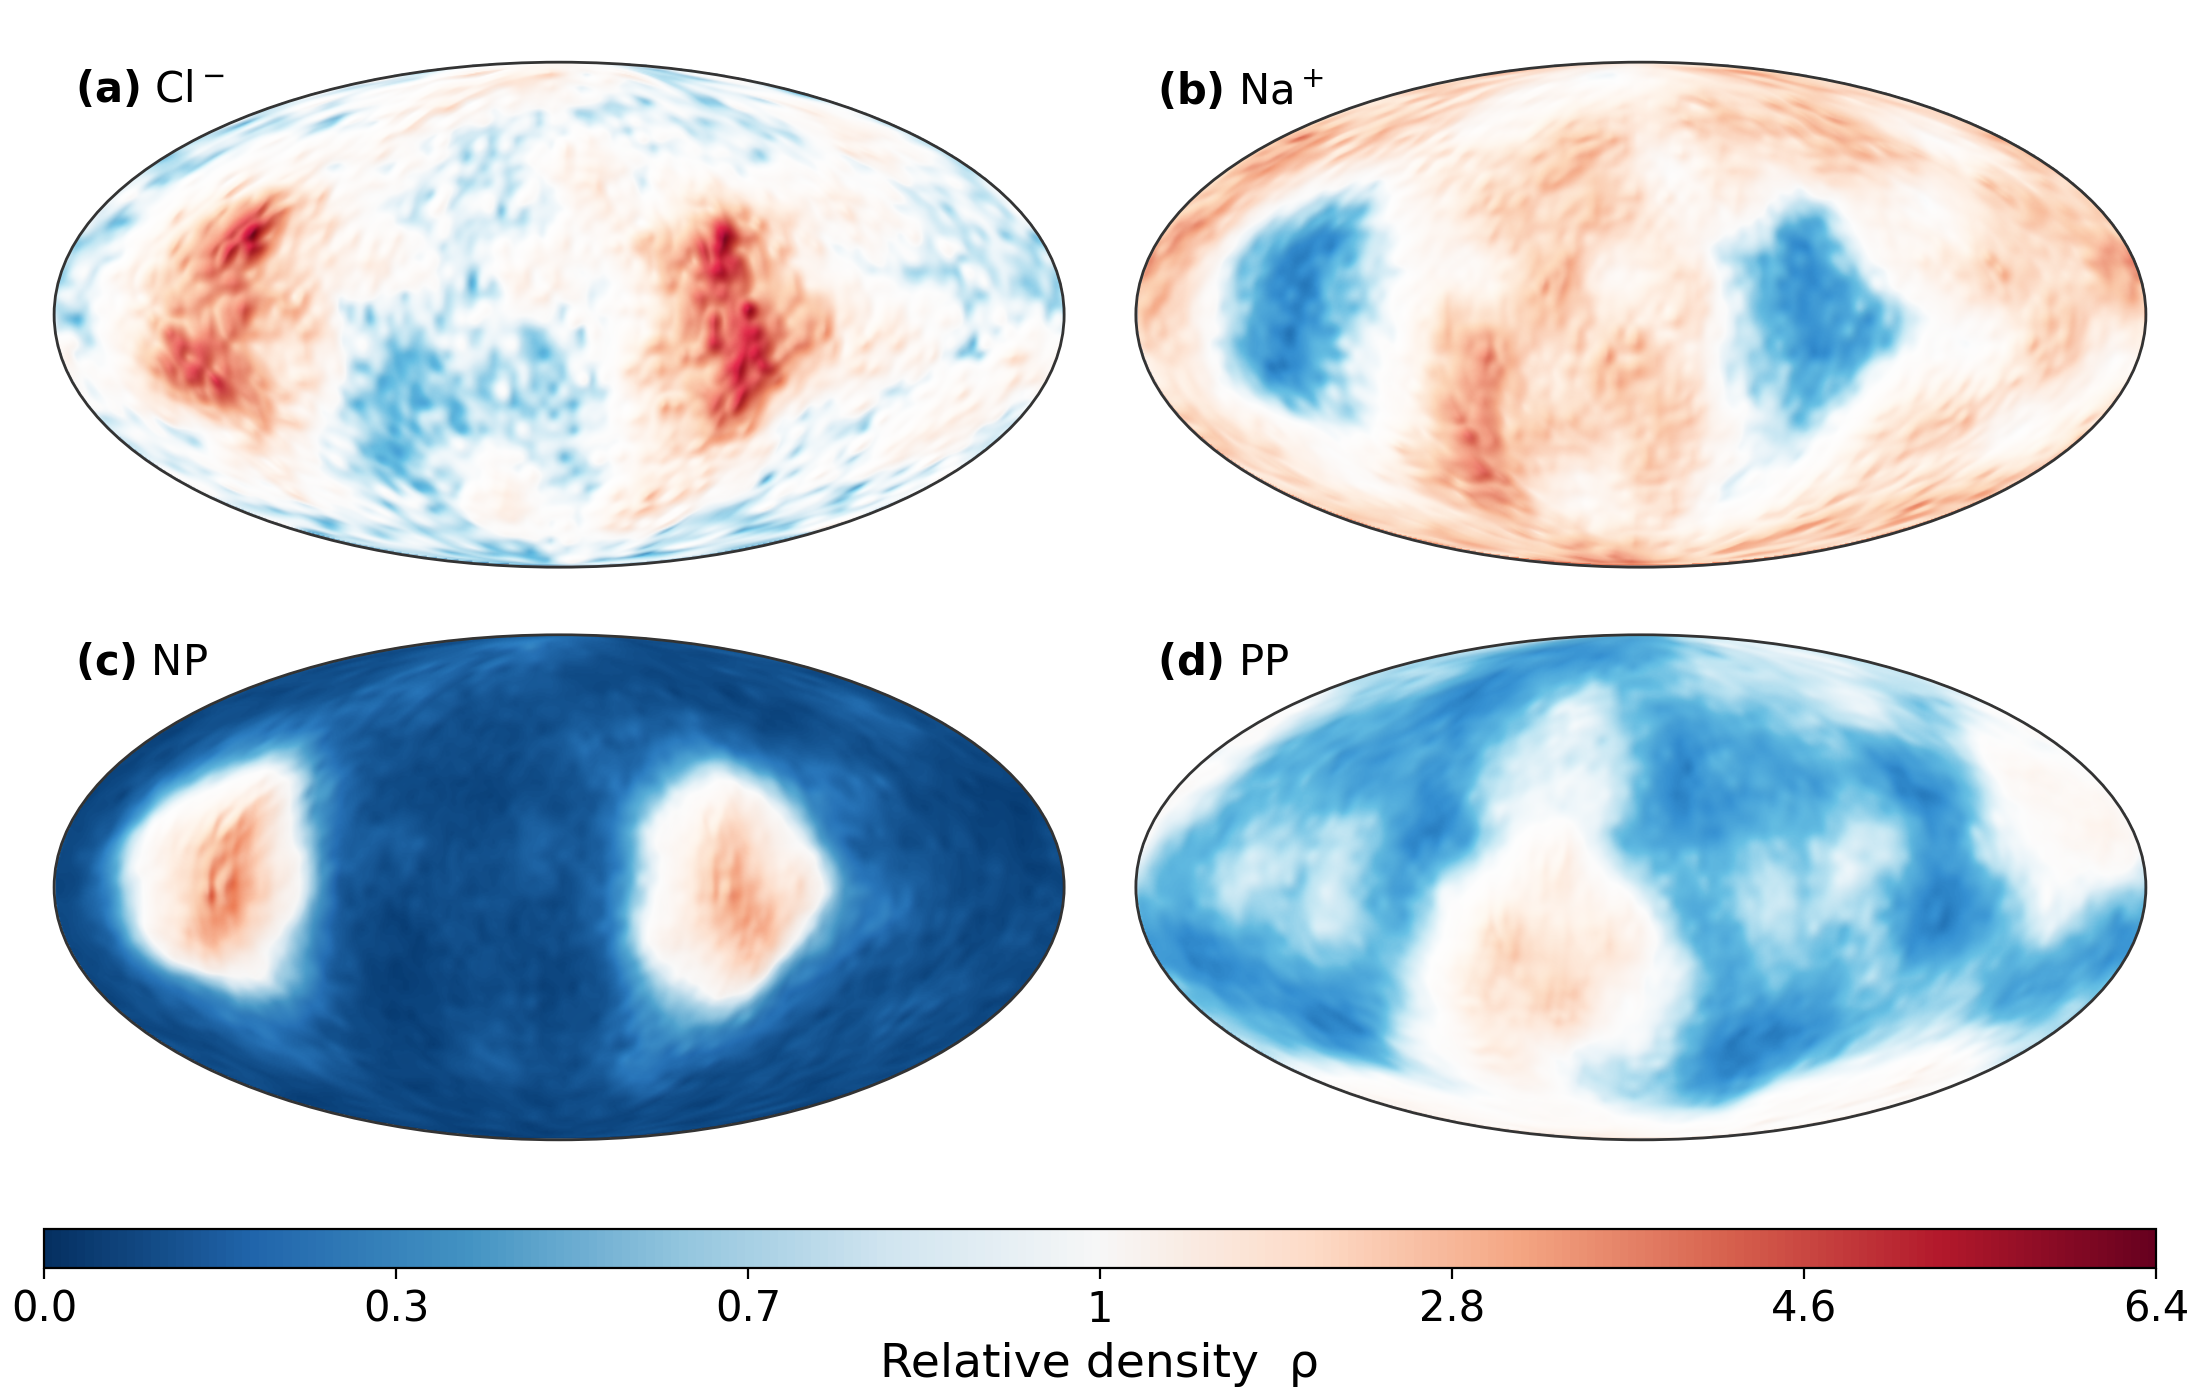
\includegraphics[width=\textwidth]{figs/quadrupolar-exp.png}
    \caption{Spatial distribution of salt ions and surface groups of neighboring
    macro-ions around each CPPM variant, projected onto a Mollweide equal-area map
    of the unit sphere.
    Local density $\rho/\rho_\mathrm{bulk}$ sampled on a spherical shell at fixed
    center-of-mass separation: $\rho = 1$ (white) = bulk; $\rho > 1$ = enrichment;
    $\rho < 1$ = depletion.
    Subpanels: (a)~chloride; (b)~sodium; (c)~NP surface groups; (d)~PP surface groups.
    The color scale is shared within each variant.
    (Top) Dipolar $\poe$ at $r = \qty{25}{\angstrom}$.
    (Bottom) Quadrupolar $\pte$ at $r = \qty{25}{\angstrom}$.}
    \label{fig:mw_sdf}
\end{figure}

\begin{figure}[htbp]
    \centering
    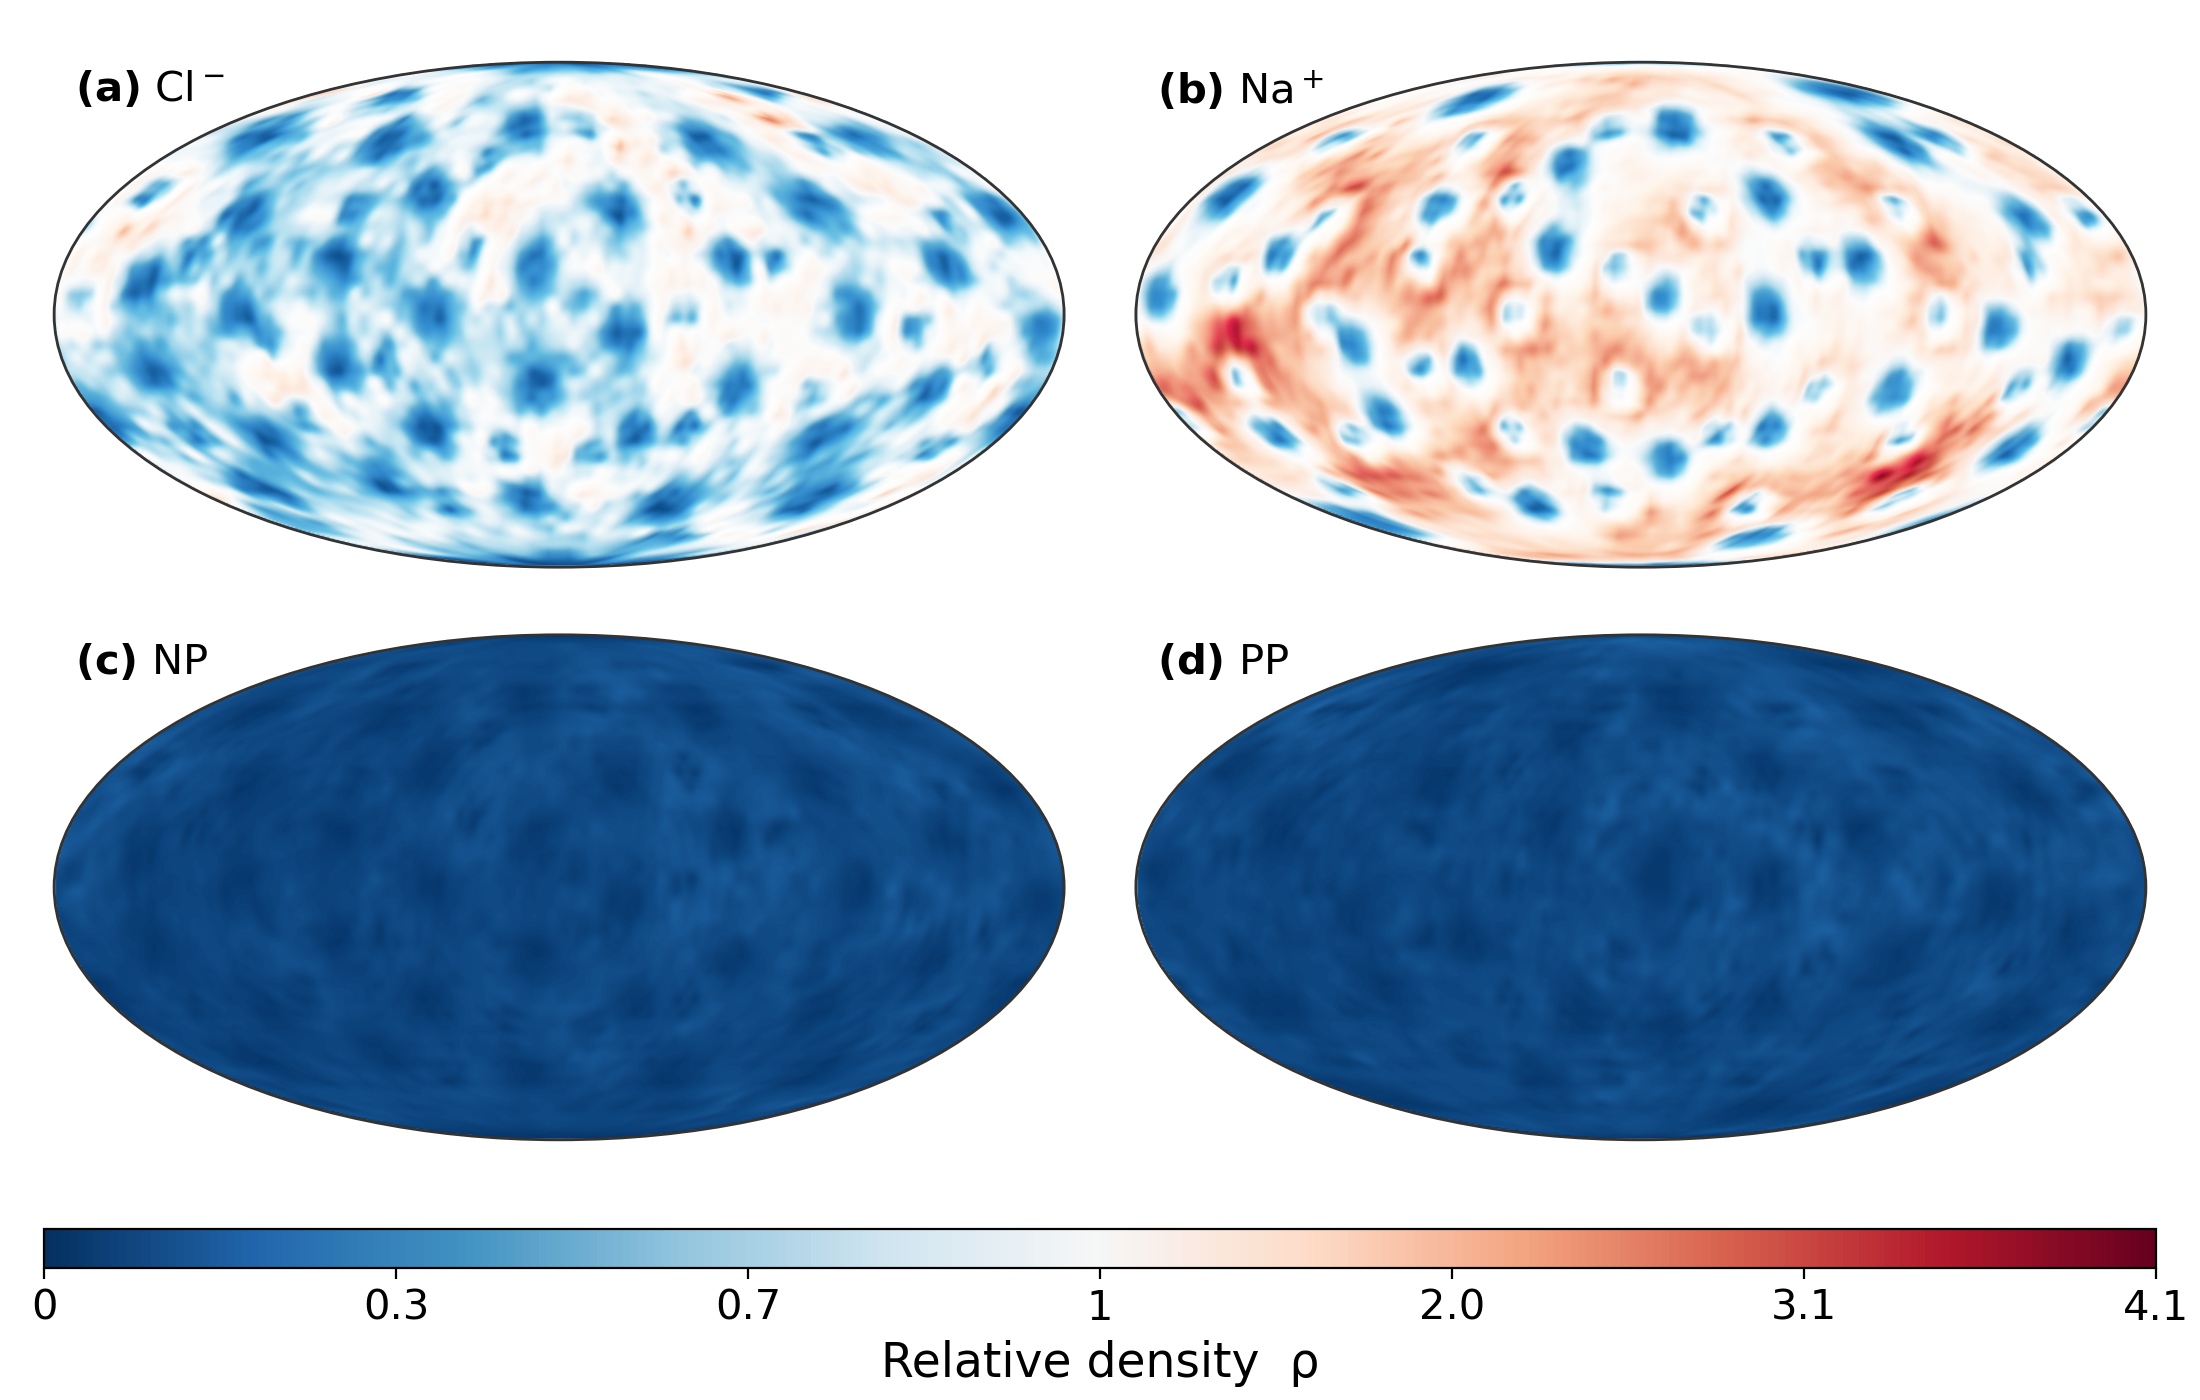
\includegraphics[width=\textwidth]{figs/isotropic-exp.png}\\[1em]
    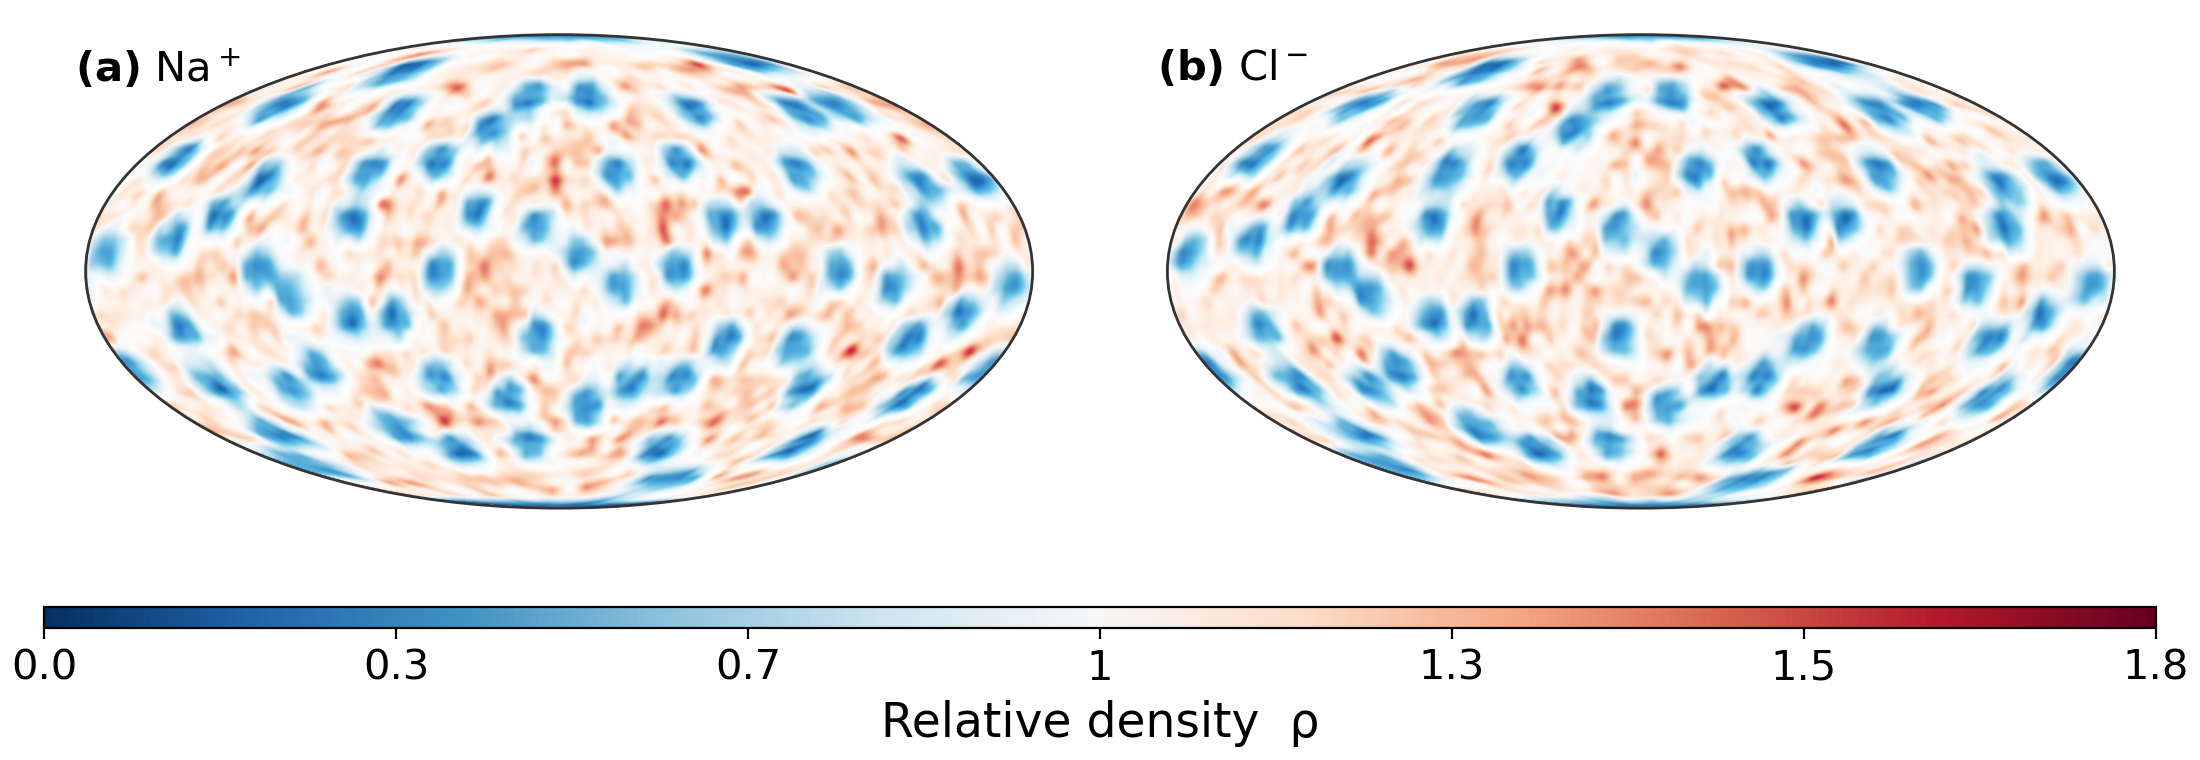
\includegraphics[width=\textwidth]{figs/neutral-exp.png}
    \caption{Same as \reffig{fig:mw_sdf} for the remaining variants.
    (Top) Isotropic $\pzz$ at $r = \qty{25}{\angstrom}$.
    (Bottom) Neutral $\pn$ at $r = \qty{23}{\angstrom}$; subpanels (c) and (d) are
    omitted because surface groups carry no charge.}
    \label{fig:mw_sdf_2}
\end{figure}

The Mollweide equal-area projections in Figs.~\ref{fig:mw_sdf}--\ref{fig:mw_sdf_2}
present the same ion-distribution data discussed in main Sec.~\ref{sec:struc_ana} in a
format that resolves the full angular structure without perspective distortion.
For the dipolar $\poe$ (\reffig{fig:mw_sdf}, top), the chloride enrichment is confined to a
single compact lobe coinciding with the positive patch (subpanel a), while sodium covers the
rest of the sphere uniformly (subpanel b).
The positive-group isosurface of neighboring macro-ions (subpanel d) appears in the
equatorial hemisphere opposite the patch, consistent with the head-to-tail pairing identified
in Sec.~\ref{esi:sec:orient_ana}.
The quadrupolar $\pte$ (\reffig{fig:mw_sdf}, bottom) shows two symmetric chloride lobes
above the two positive patches and four well-localized positive-group spots, reflecting the
two-fold symmetry of the anti-aligned quadrupolar ordering.
For the isotropic $\pzz$ (\reffig{fig:mw_sdf_2}, top) both ion species are nearly uniform
across the sphere, with sodium enrichment everywhere and a diffuse, patternless chloride
distribution.
The neutral $\pn$ (\reffig{fig:mw_sdf_2}, bottom) shows both species uniformly and weakly
distributed, confirming the absence of any electrostatically driven selectivity.

% ─────────────────────────────────────────────────────────────────────────────
\section{Debye length scan\label{esi:sec:dl_scan}}
% ─────────────────────────────────────────────────────────────────────────────

\begin{figure}[htbp]
    \centering
    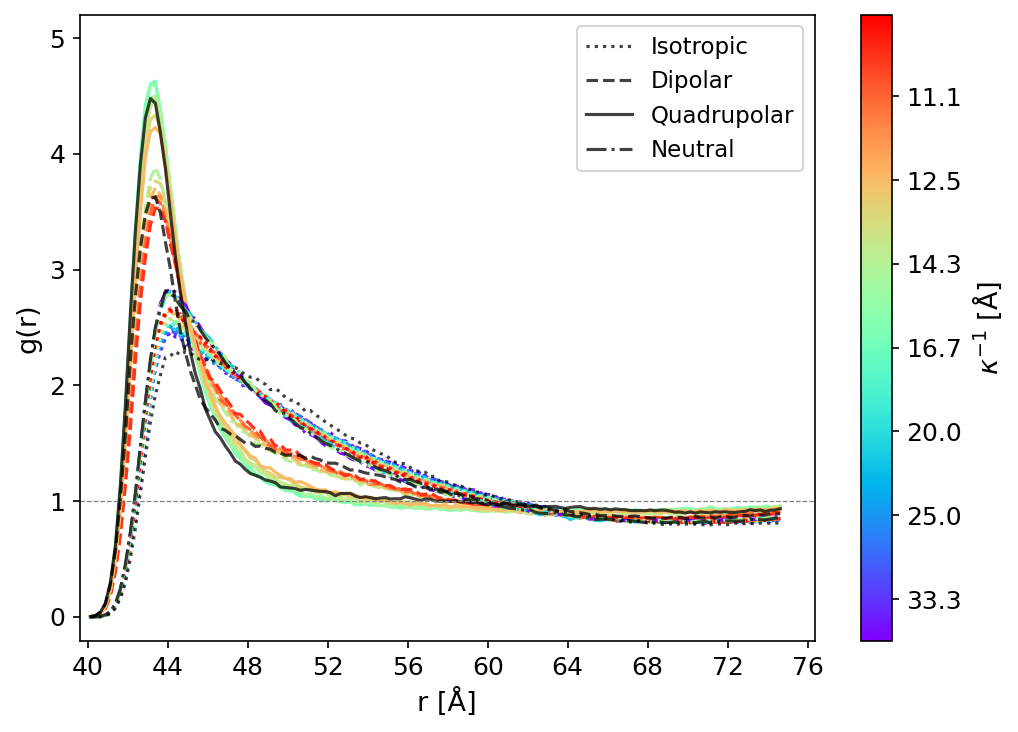
\includegraphics[width=\textwidth]{figs/rdf_overlay_combined.png}
    \caption{Center-of-mass $g(r)$ for the three charged variants over the full $\dl$
    scan from implicit-ion simulations.
    $\pzz$ (dotted), $\poe$ (dashed), $\pte$ (solid).
    Line color encodes $\dl$ (rainbow bar: violet = weak screening, large $\dl$;
    red = strong screening, small $\dl$).
    Black lines: explicit-ion reference.
    Shaded bands: mean $\pm$ SEM.}
    \label{fig:gofr_com}
\end{figure}

\begin{figure}[htbp]
    \centering
    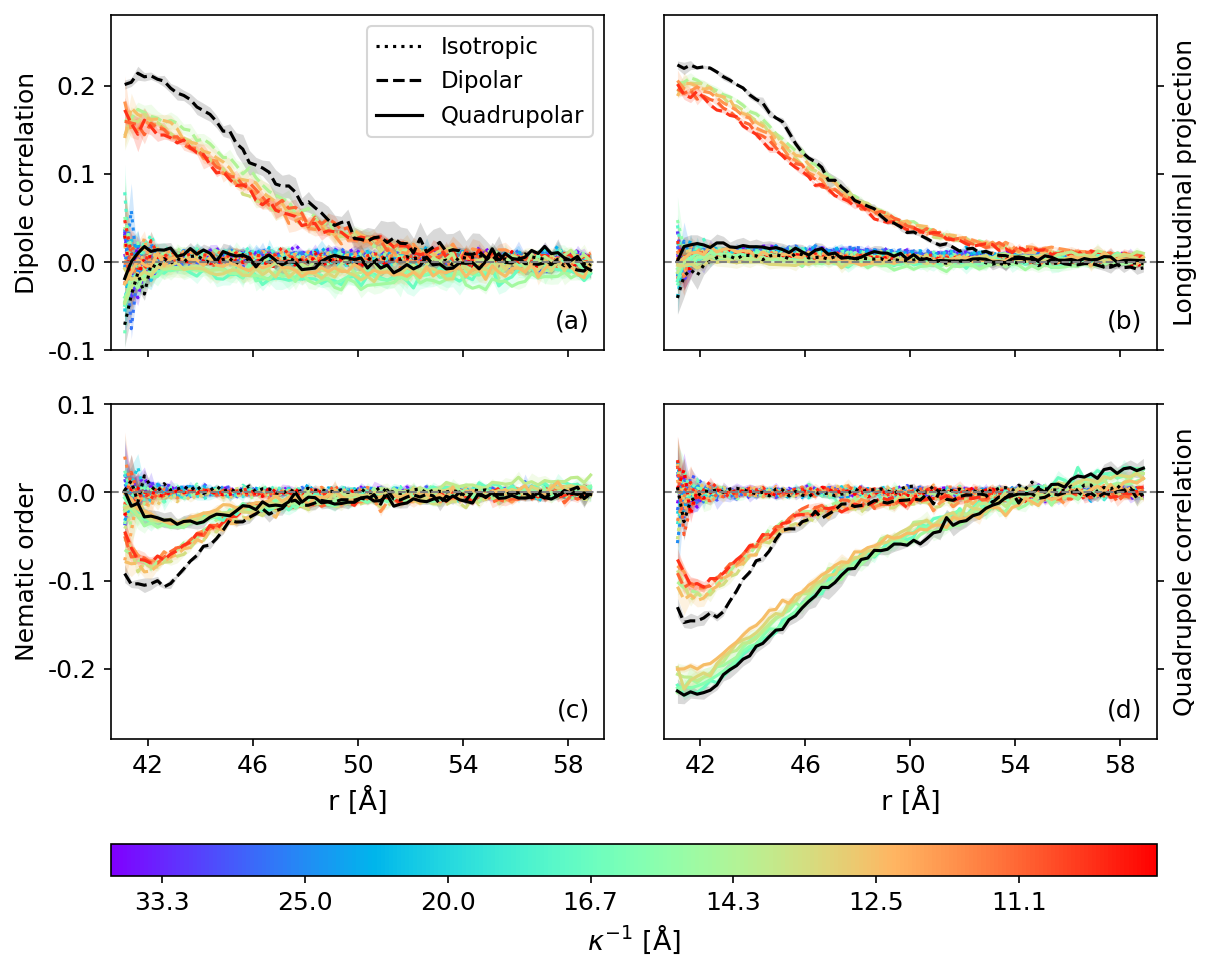
\includegraphics[width=\textwidth]{figs/multipole_corr_combined.png}
    \caption{Orientational pair correlations for the three charged variants over the
    full $\dl$ scan.
    (a)~$\langle\hat{\mu}_i\cdot\hat{\mu}_j\rangle$;
    (b)~$\langle(\hat{\mu}_i\cdot\hat{r}_{ij})(\hat{\mu}_j\cdot\hat{r}_{ij})\rangle$;
    (c)~$\langle P_2(\cos\theta_{ij})\rangle$;
    (d)~$\langle\hat{\mathbf{Q}}_i{:}\hat{\mathbf{Q}}_j\rangle$.
    Rainbow color bar encodes $\dl$; black lines: explicit-ion reference;
    shaded bands: mean $\pm$ SEM.}
    \label{fig:mp_corr}
\end{figure}

\begin{figure}[htbp]
    \centering
    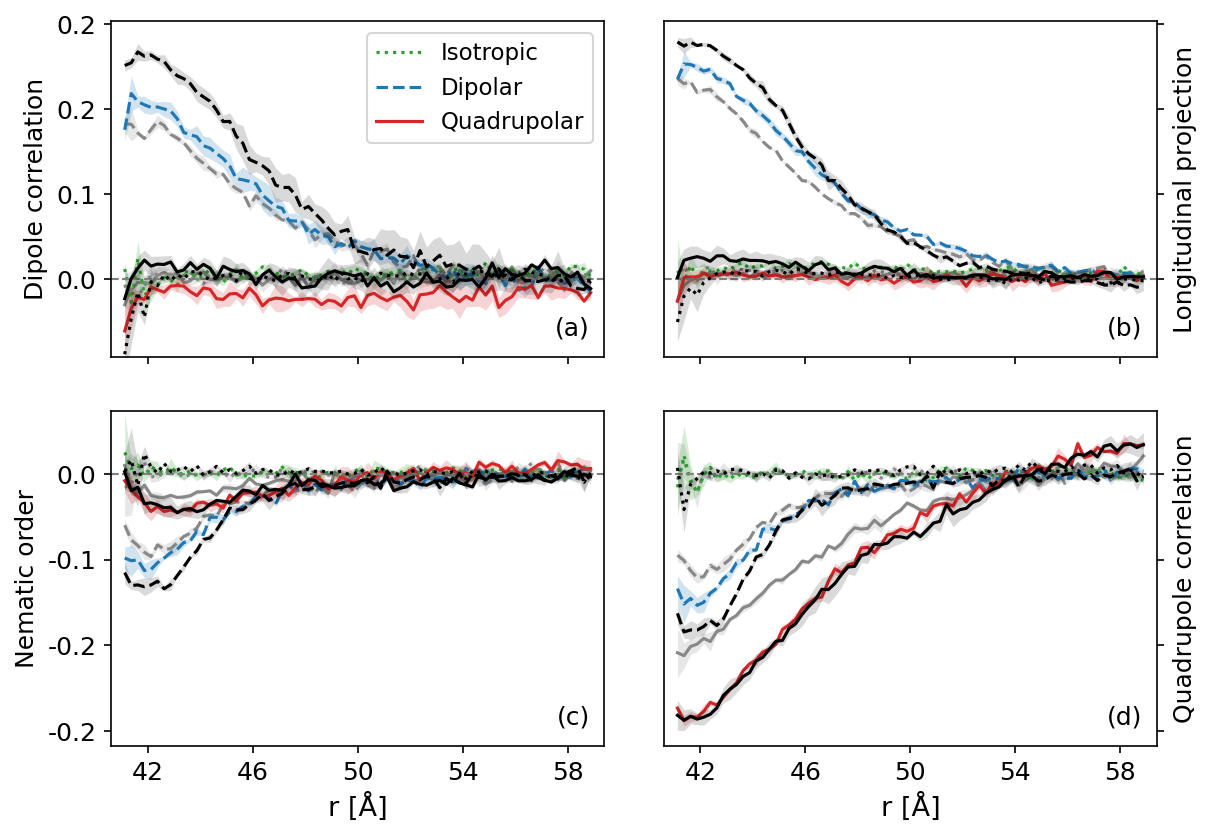
\includegraphics[width=\textwidth]{figs/multipole_corr_best_kappa.png}
    \caption{Orientational pair correlations at the best-fit screening length $\dl_*$
    (colored lines, one per variant) and at the theoretically predicted $\dl_\mathrm{th}$
    (gray lines), compared with the explicit-ion reference (black lines).
    Panel layout as in \reffig{fig:mp_corr}.
    Shaded bands: mean $\pm$ SEM.}
    \label{fig:mp_corr_best}
\end{figure}

\begin{figure}[htbp]
    \centering
    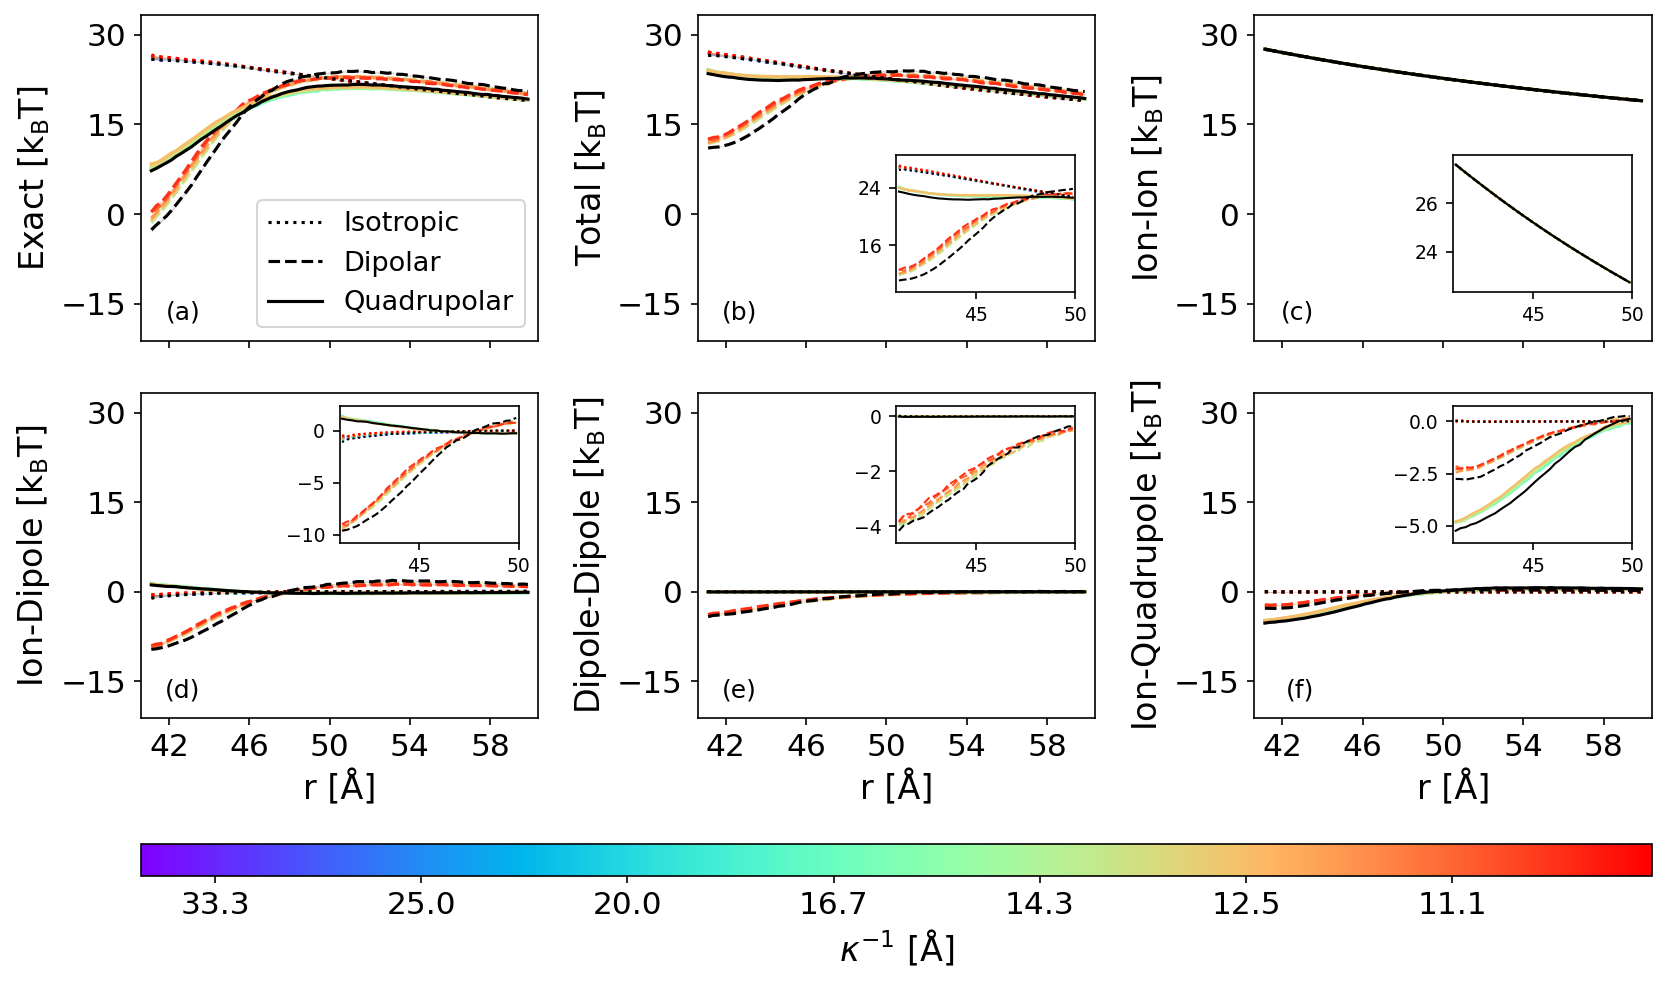
\includegraphics[width=\textwidth]{figs/multipole_energy_combined.png}
    \caption{Distance-dependent pairwise energy contributions over the full $\dl$ scan.
    Panel layout as in \reffig{fig:multi_ene_exp} with an individual energy axis per panel.
    Rainbow color bar encodes $\dl$; black lines: explicit-ion reference;
    shaded bands: mean $\pm$ SEM.
    Insets: zoomed view of the contact region ($r \le \qty{50}{\angstrom}$).}
    \label{fig:mp_ene}
\end{figure}

\begin{figure}[htbp]
    \centering
    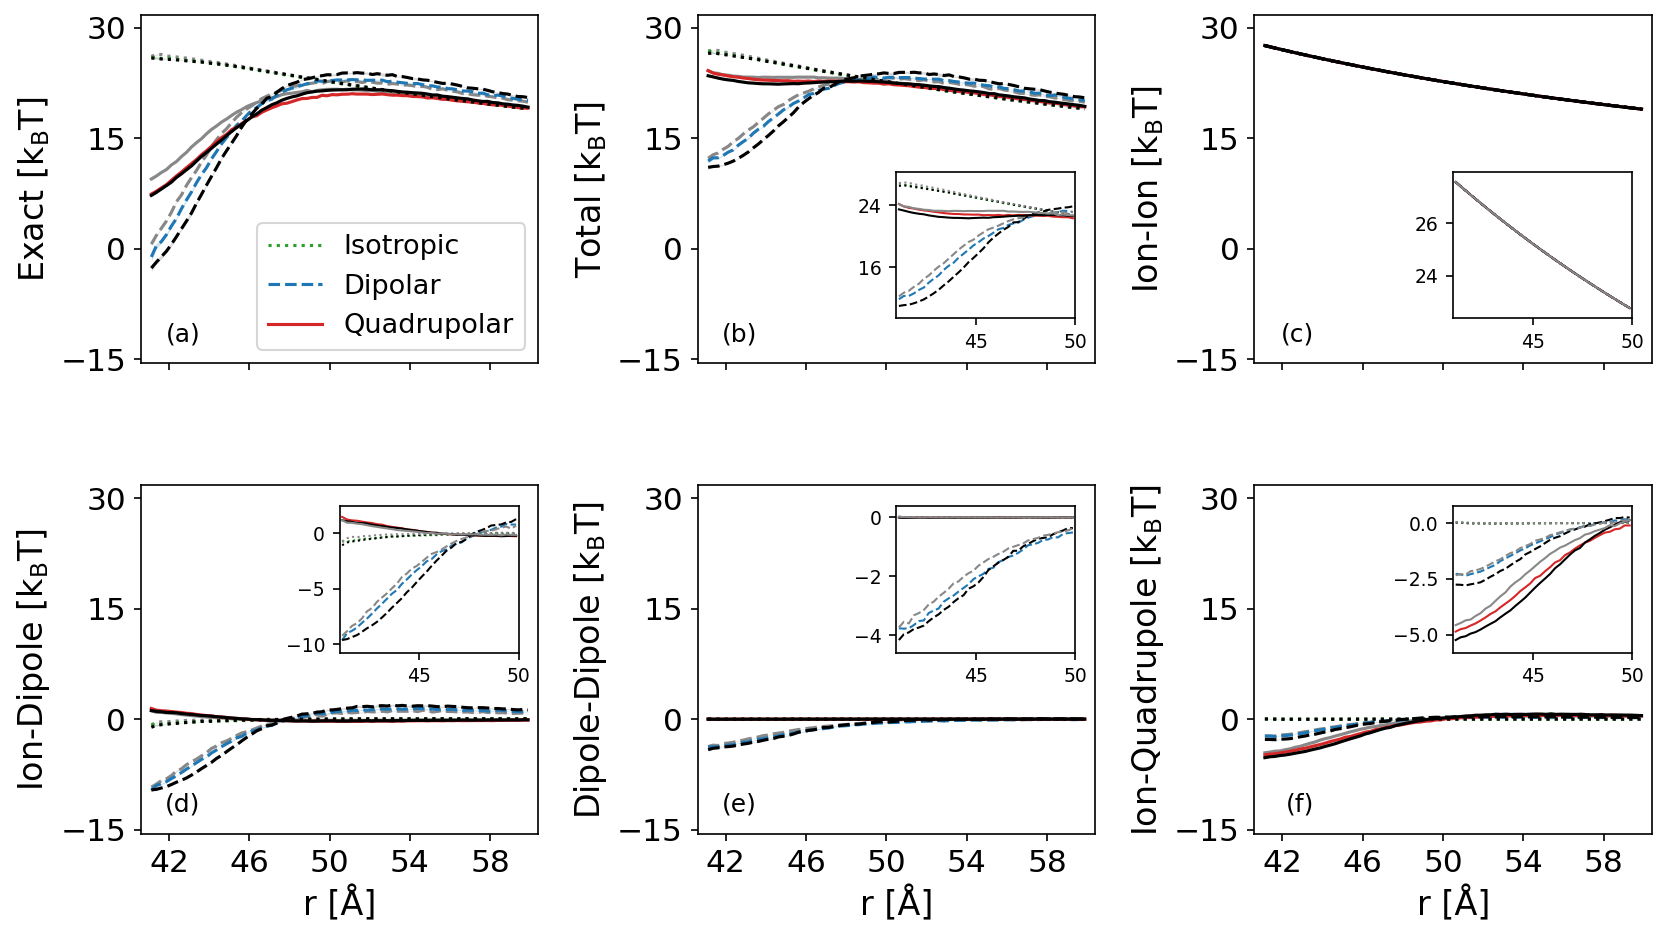
\includegraphics[width=\textwidth]{figs/multipole_energy_best_kappa.png}
    \caption{Pairwise energy contributions at $\dl_*$ (colored) and $\dl_\mathrm{th}$
    (gray) vs.\ the explicit-ion reference (black).
    Panel layout as in \reffig{fig:multi_ene_exp}.
    Shaded bands: mean $\pm$ SEM.
    Insets: zoomed view of the contact region ($r \le \qty{50}{\angstrom}$).}
    \label{fig:mp_ene_best}
\end{figure}

\reffig{fig:gofr_com} shows the full dependence of $g(r)$ on $\dl$ for the three charged
variants.
For the dipolar $\poe$ and quadrupolar $\pte$, the peak height tracks monotonically with
$\dl$: stronger screening (smaller $\dl$) increases the peak because the reduced long-range
repulsion allows closer approach.
For the isotropic $\pzz$, the peak height also increases with stronger screening, but every
implicit-ion $g(r)$ systematically overestimates the explicit-ion reference across the entire
scanned range ($\dl = 10$--$\qty{38}{\angstrom}$), confirming the fundamental limitation of
the implicit-ion model for this variant discussed in main Sec.~\ref{sec:impl}.

Figures~\ref{fig:mp_corr}--\ref{fig:mp_corr_best} extend the comparison to orientational
correlations.
The evolution of the dipole--dipole and quadrupole--quadrupole correlations with $\dl$
closely tracks the $g(r)$ peak: stronger screening amplifies orientational order, and the
optimal $\dl_*$ recovers not only the correct $g(r)$ peak height but also the correct
orientational order for $\poe$ and $\pte$ (main Sec.~\ref{sec:best_kappa}).

Figures~\ref{fig:mp_ene}--\ref{fig:mp_ene_best} compare the pairwise multipole energy
components across the $\dl$ scan and at $\dl_*$.
The implicit-ion ion--ion term $u_{ii}$ (panel c in both figures) varies strongly with
$\dl$ and converges to the explicit-ion reference at the best-fit screening length for
$\poe$ and $\pte$, while remaining discrepant for $\pzz$ at all values tested.

% ─────────────────────────────────────────────────────────────────────────────
\section{Energy convergence\label{esi:sec:econv}}
% ─────────────────────────────────────────────────────────────────────────────

Figures~\ref{fig:e_exp}--\ref{fig:e_sim_neu} show the running-mean total energy
$U/k_\mathrm{B}T$ as a function of Monte Carlo sweeps for all simulations reported in
the main article.
The stabilization of the cumulative mean (thick lines) confirms convergence for all
systems and replicas.

\begin{figure}[htbp]
    \centering
    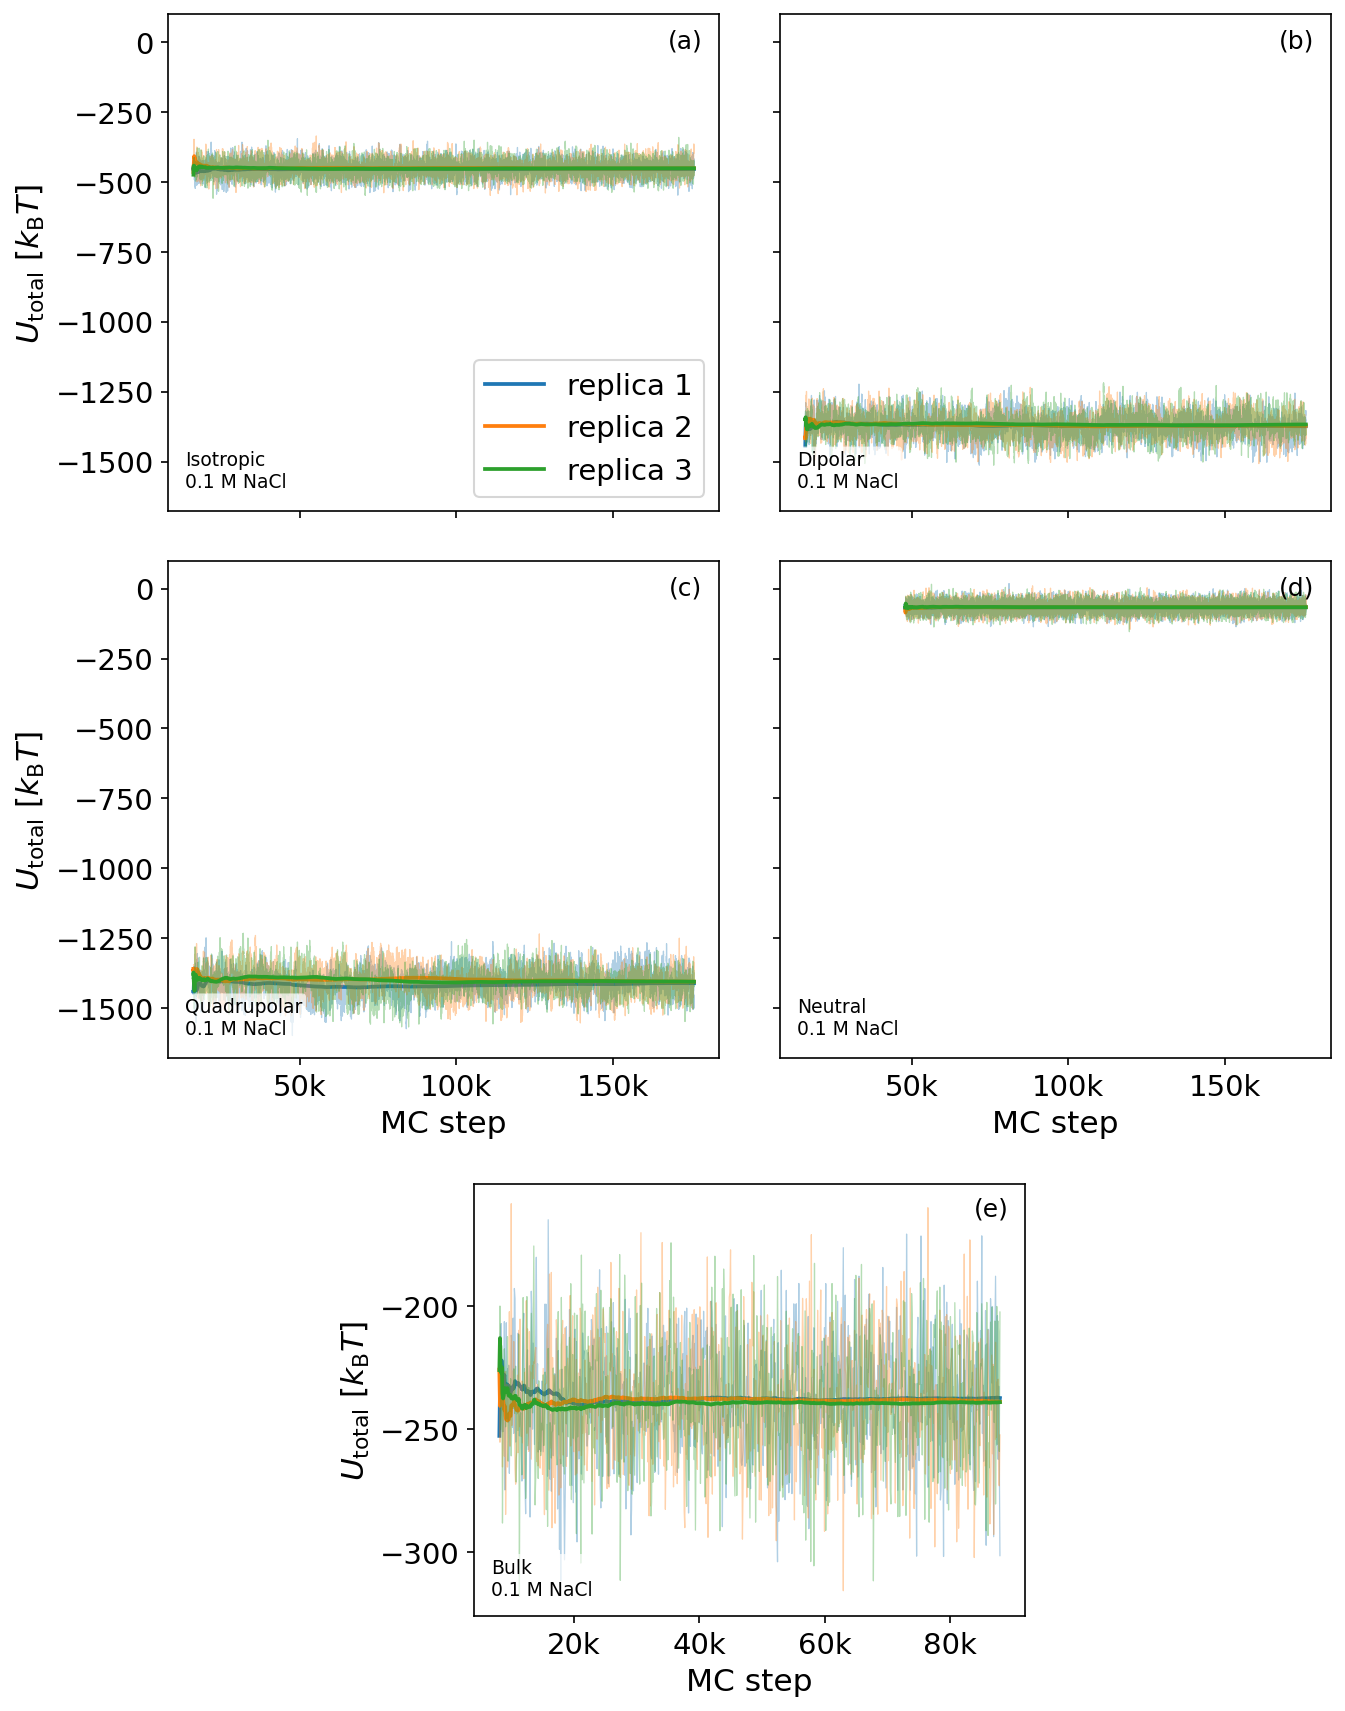
\includegraphics[width=\textwidth]{figs/energy_convergence_explicit.png}
    \caption{Total energy vs.\ MC sweeps for the explicit-ion simulations:
    (a)~$\pzz$, (b)~$\poe$, (c)~$\pte$, (d)~$\pn$, (e)~bulk \ce{NaCl}.
    Thin lines: raw trace; thick lines: running cumulative mean.
    Colors distinguish replicas (blue, orange, green).
    Panels (a)--(d) share a common energy axis; (e) has its own scale.}
    \label{fig:e_exp}
\end{figure}

\begin{figure}[htbp]
    \centering
    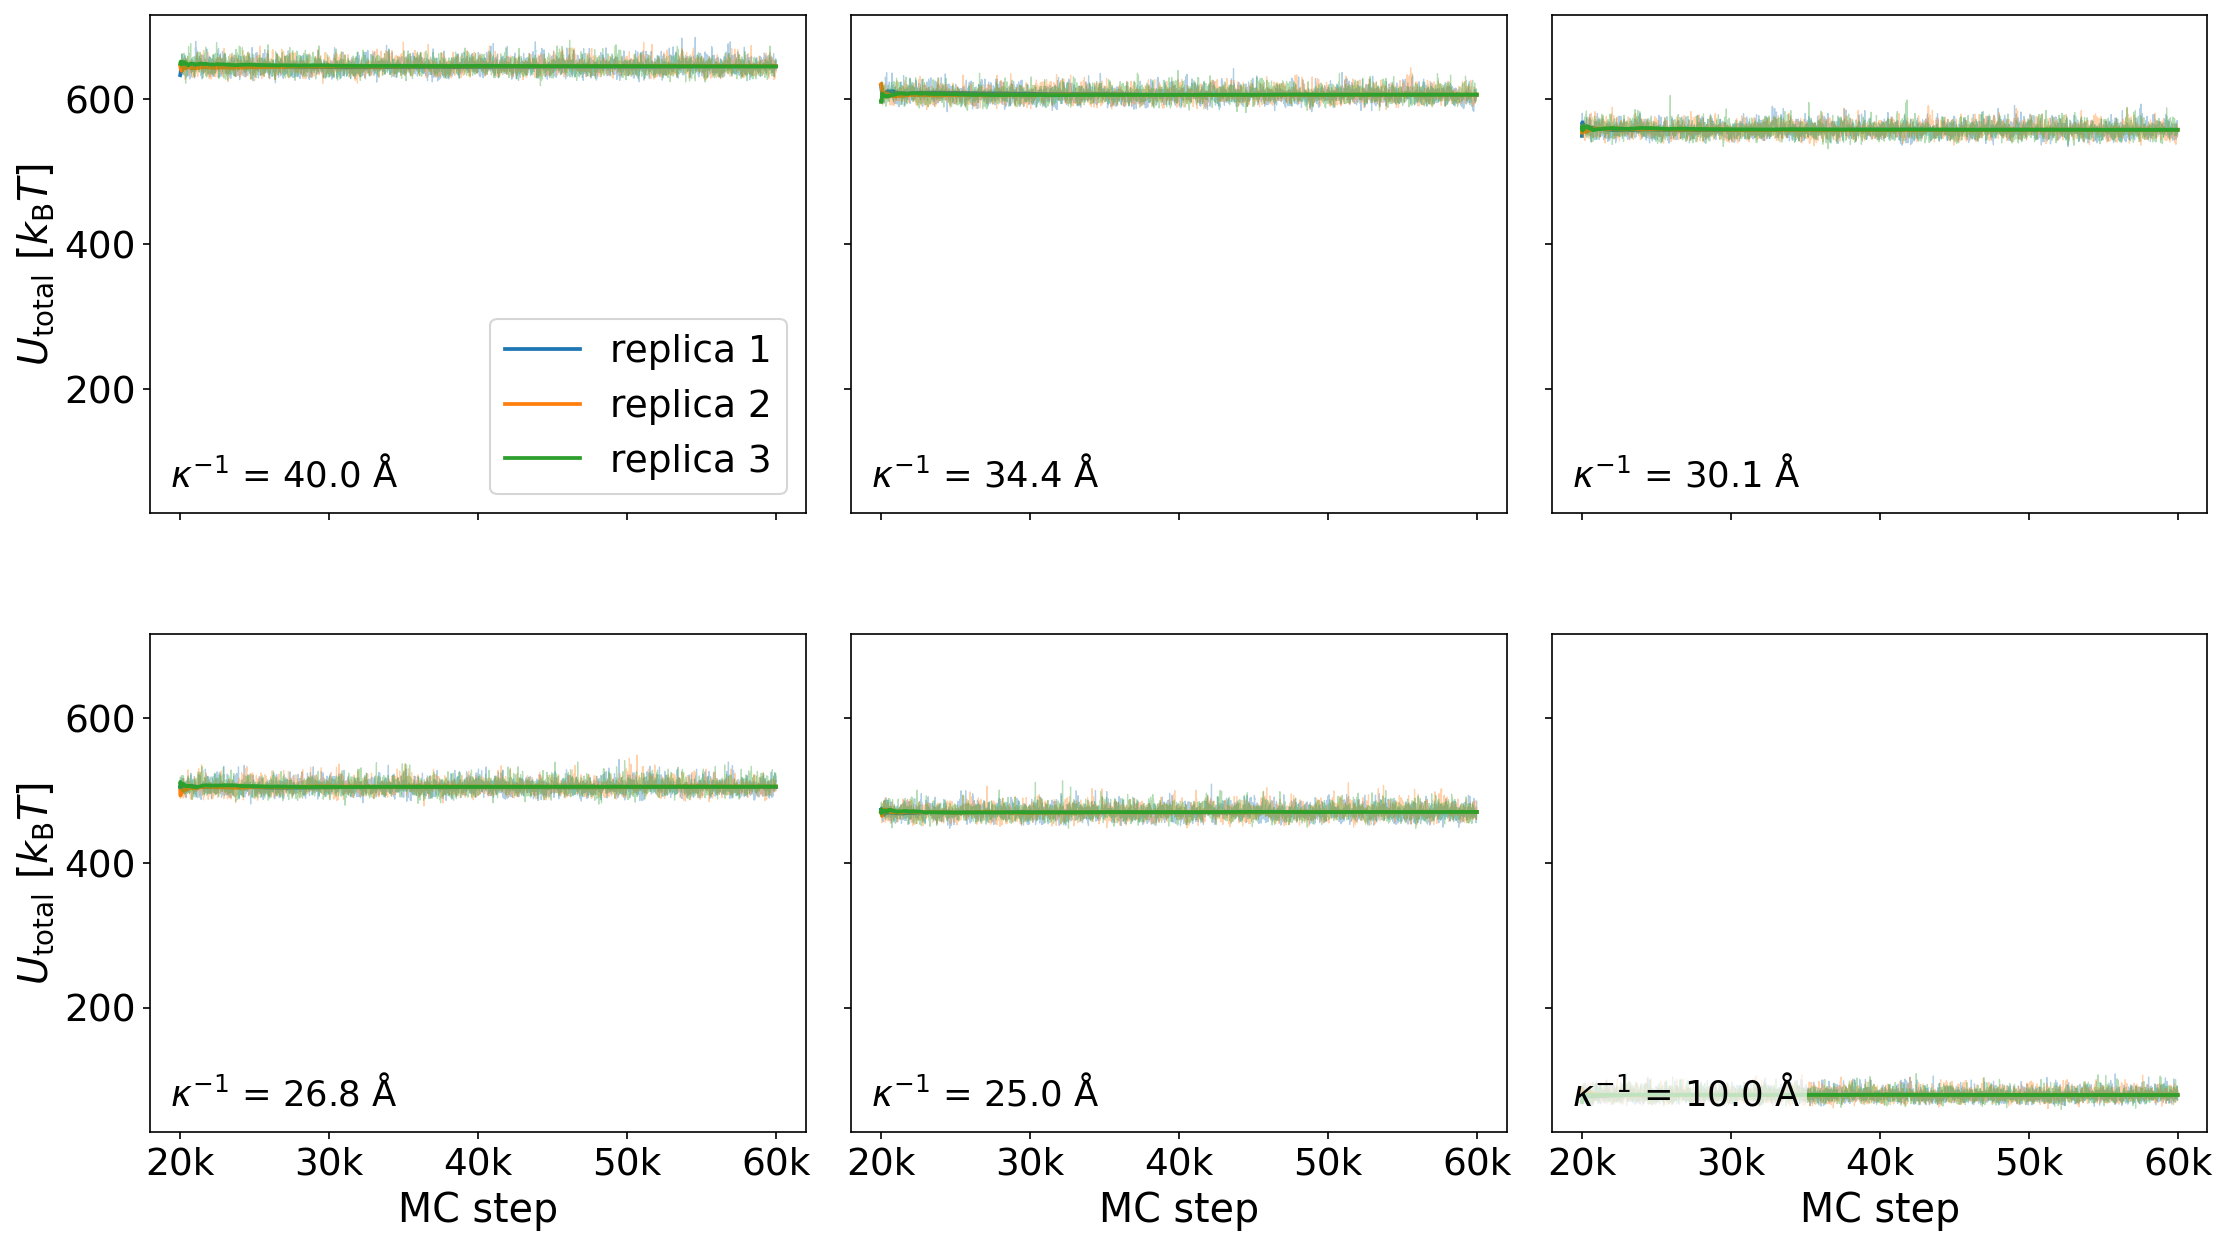
\includegraphics[width=\textwidth]{figs/energy_convergence_isotropic.png}
    \caption{Total energy vs.\ MC sweeps for the implicit-ion simulations of $\pzz$.
    Each panel shows one value of $\dl$ (indicated in the lower-left corner).
    Thin lines: raw trace; thick lines: running cumulative mean.
    Colors distinguish replicas.
    All panels share a common energy axis.}
    \label{fig:e_imp_iso}
\end{figure}

\begin{figure}[htbp]
    \centering
    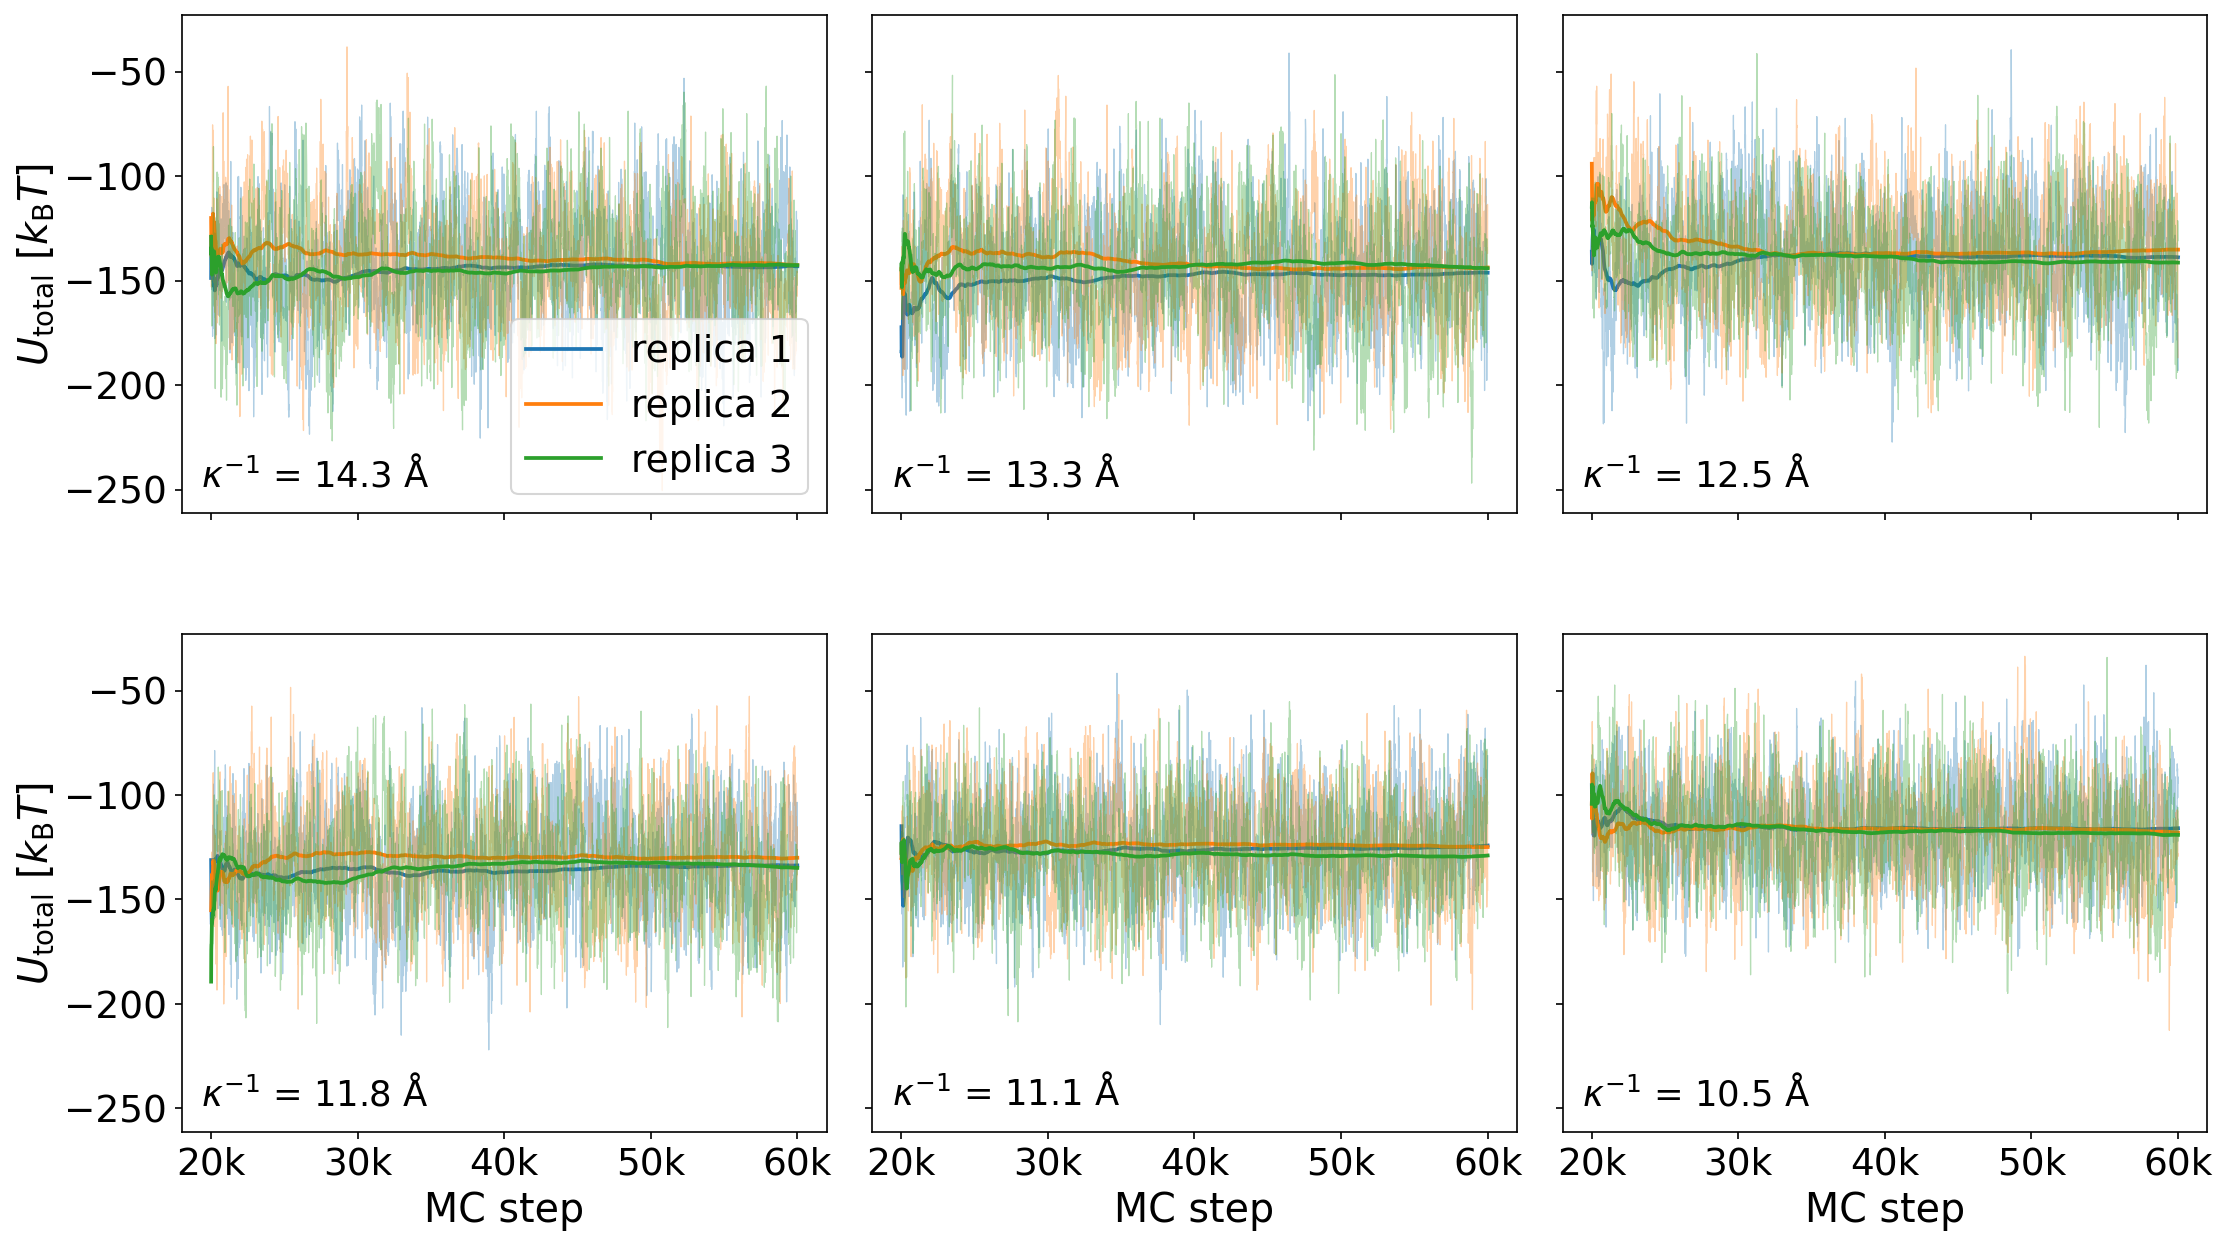
\includegraphics[width=\textwidth]{figs/energy_convergence_dipolar.png}
    \caption{As \reffig{fig:e_imp_iso} for $\poe$.}
    \label{fig:e_imp_dip}
\end{figure}

\begin{figure}[htbp]
    \centering
    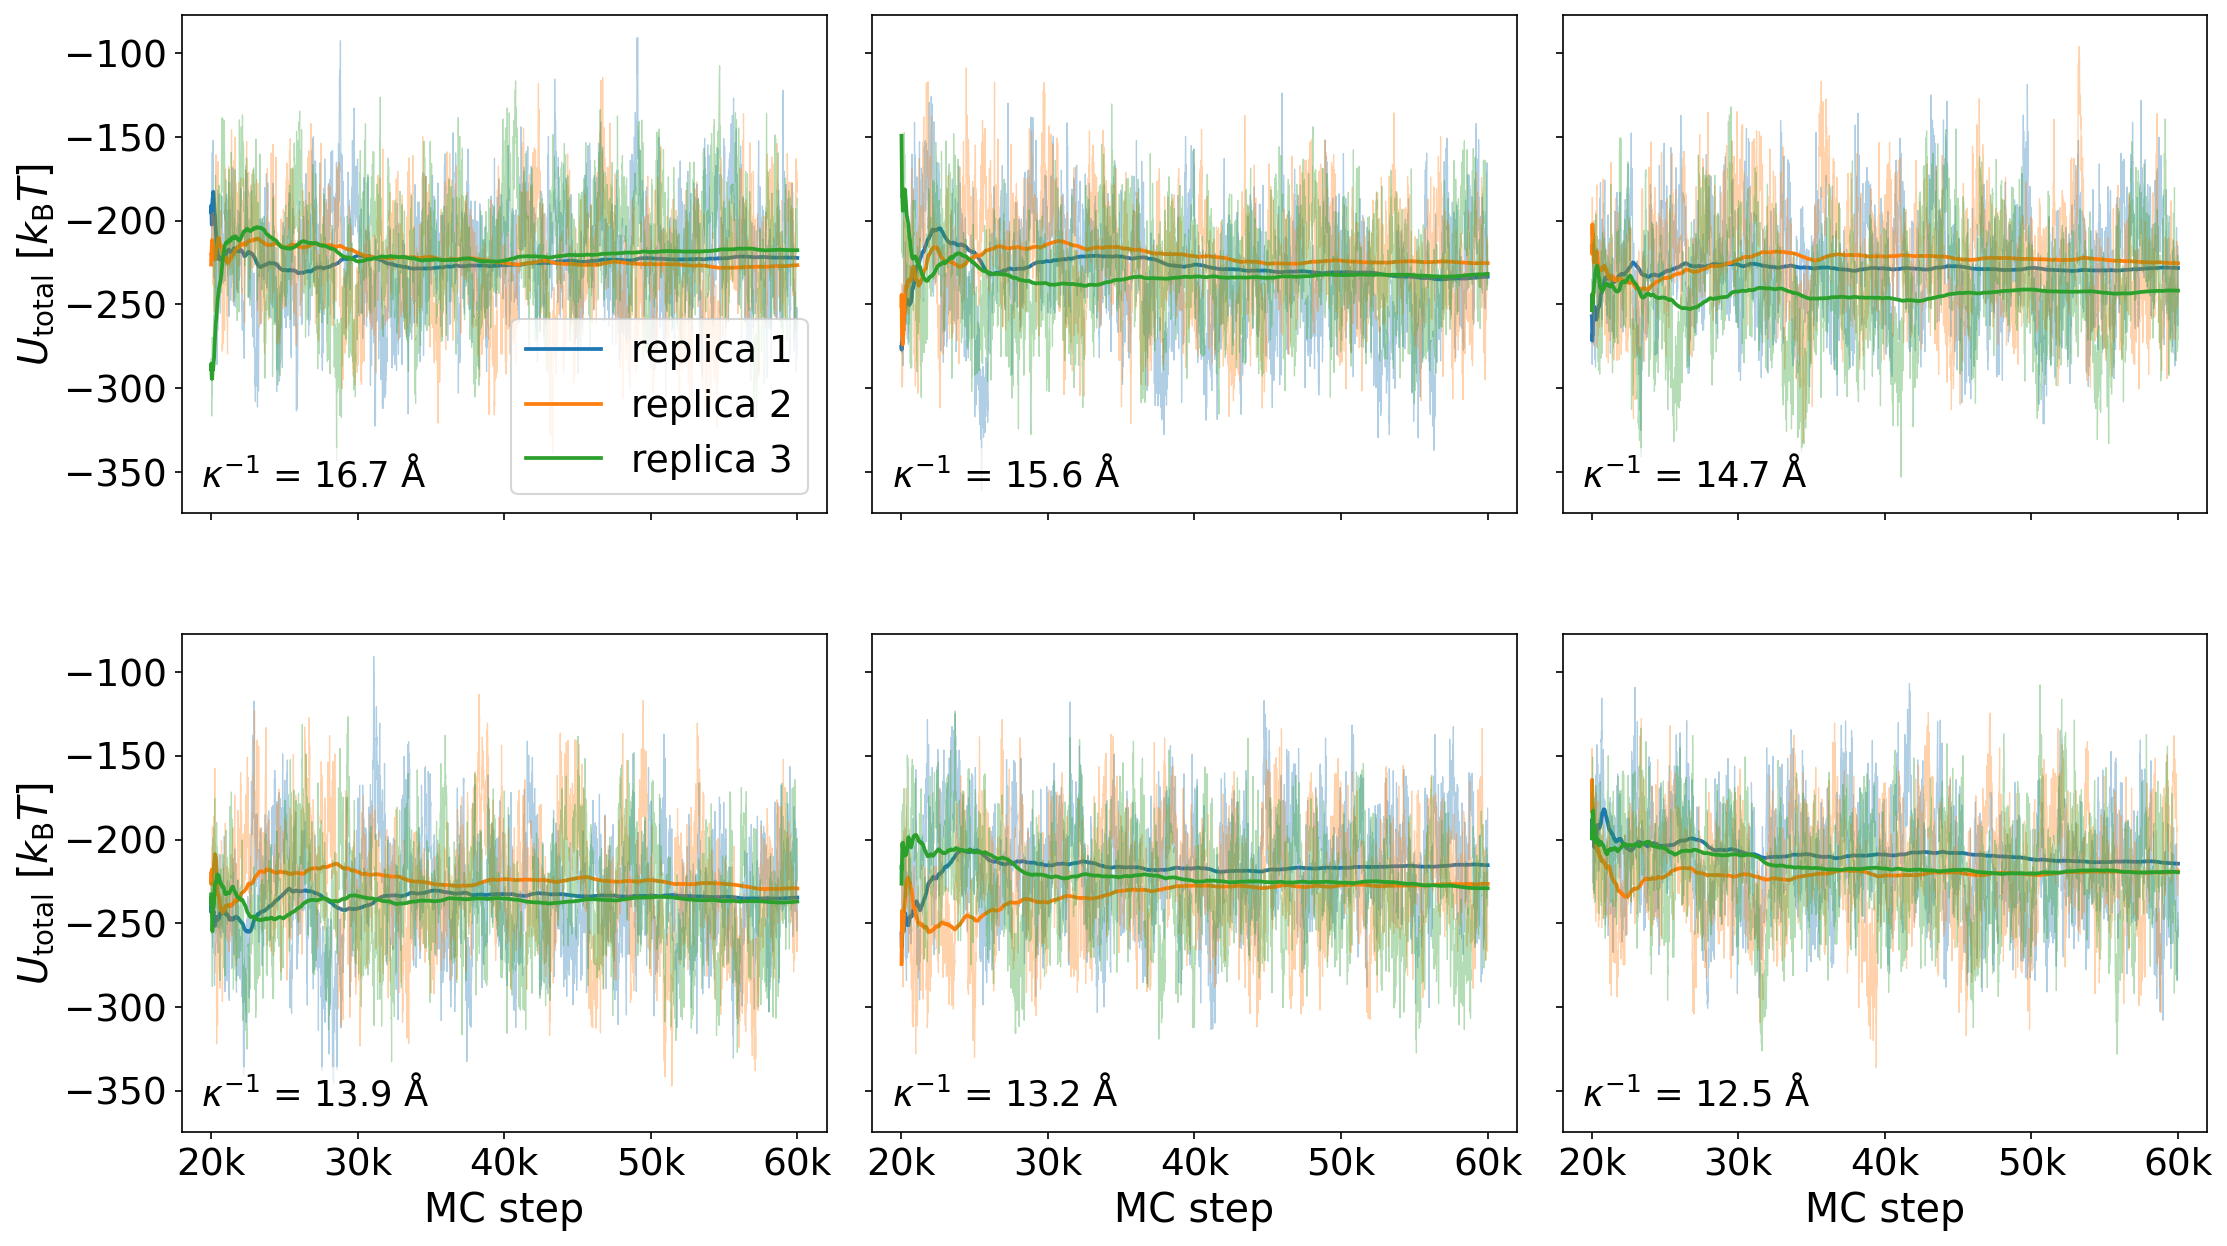
\includegraphics[width=\textwidth]{figs/energy_convergence_quadrupolar.png}
    \caption{As \reffig{fig:e_imp_iso} for $\pte$.}
    \label{fig:e_sim_quad}
\end{figure}

\begin{figure}[htbp]
    \centering
    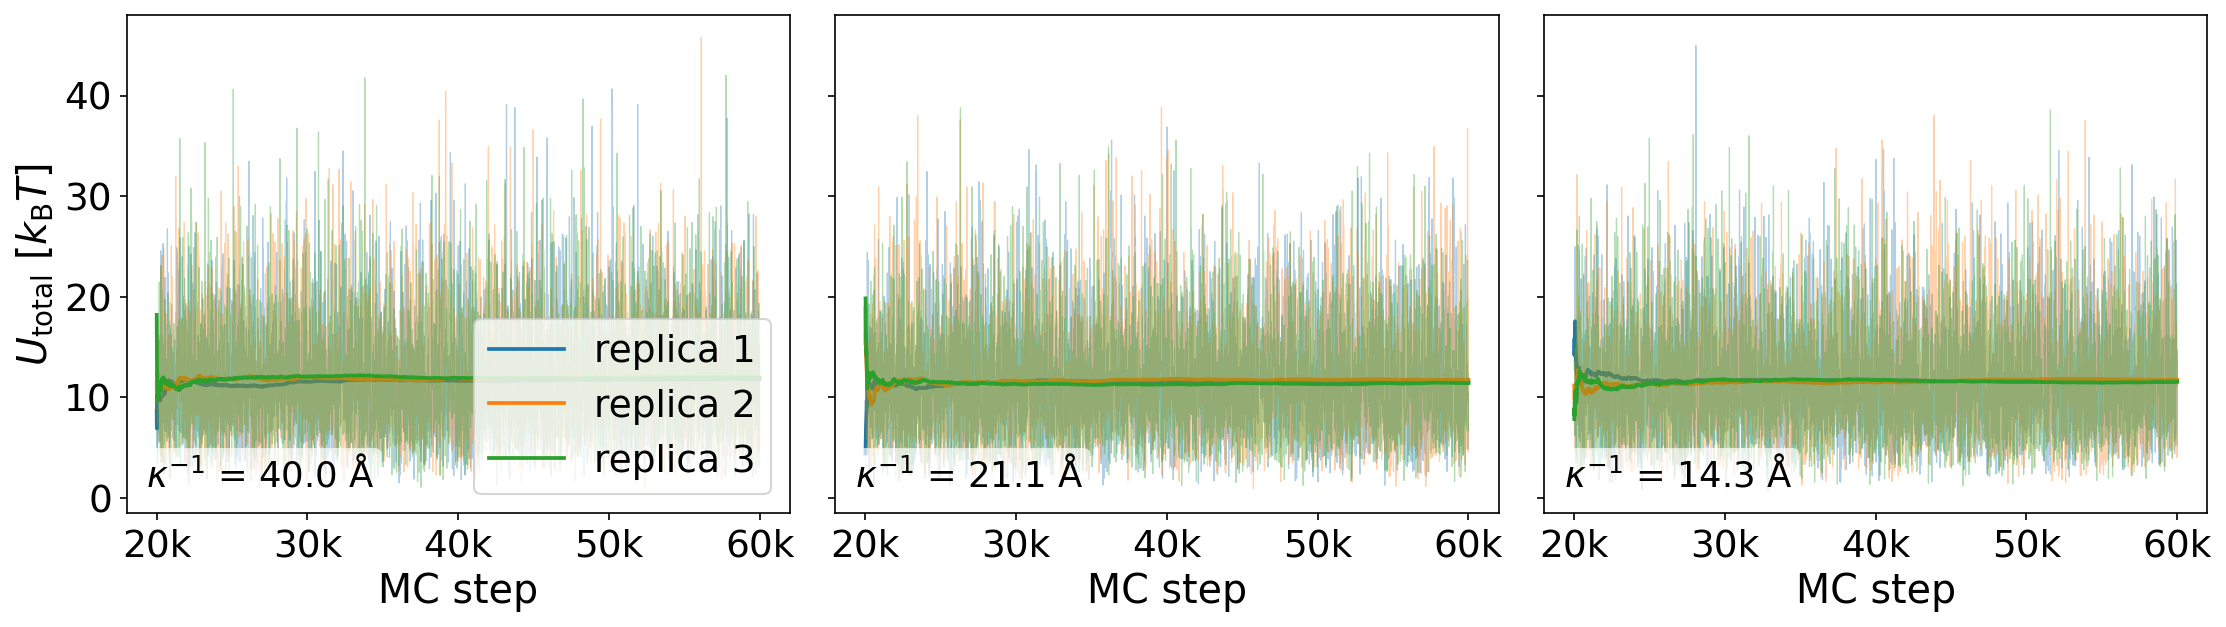
\includegraphics[width=\textwidth]{figs/energy_convergence_neutral.png}
    \caption{As \reffig{fig:e_imp_iso} for $\pn$.}
    \label{fig:e_sim_neu}
\end{figure}

\bibliographystyle{unsrt}
\bibliography{pmc}

\end{document}
